%!TEX root = ../my_thesis.tex
\section{Decay-time fit to data}
\label{sec:datafit}

The \CP~coefficients $S_{f}$ and $S_{\bar f}$ are determined from an unbinned maximum likelihood fit
where each candidate is weighted with the \emph{sWeights} extracted from the mass fit described in
Sec.~\ref{sec:fitB}. Hence, the total PDF is given solely by the PDF \mbox{$f(t, d_{\rm OS}, d_{\rm SS} , \eta_{\rm OS}, \eta_{\rm SS}, q)$} describing the signal distribution. This is proportional to
\begin{equation}
	\label{eq:fulltimepdf}
       a(t) \int dt' \mathcal R(t-t') P(t' | d_{\rm OS}, d_{\rm SS}, \eta_{\rm OS}, \eta_{\rm SS}, q) E^{\rm OS}(\eta_{\rm OS}) E^{\rm SS}(\eta_{\rm SS}) D^{\rm OS}(d_{\rm OS}) D^{\rm SS}(d_{\rm SS}) Q(q),
\end{equation}
where $R(t-t')$ is the Gaussian resolution
function, $a(t)$ is the acceptance function, $E^{\rm OS}(\eta_{\rm OS})$ and $E^{\rm SS}(\eta_{\rm SS})$ are the PDFs of the predicted mistag probability of the taggers, $D^{\rm OS}(d_{\rm OS})$ and $D^{\rm SS}(d_{\rm SS})$ are the PDFs of the decision of the taggers, and
$Q(q)$ is the PDF of the final states.
%The convolution integral is optimized by following the strategy described in Ref.~\cite{spline}.
The function $P^(t |  d_{\rm OS}, d_{\rm SS}, \eta_{\rm OS}, \eta_{\rm SS}, q)$ represents the expected decay-time distribution
for a \Bz~or a \Bzb~decaying into a $\Dm\pi^+$ or $\Dp\pi^-$ final state. This is conditional on the tagging
decisions $d_{i}$, the mistag probabilities $\eta_{i}$ and the final state $q$, and it contains the decay rates of
Eqs.~\ref{eq:decay-rate-Bf}--\ref{eq:decay-rate-Bbfb}. A detailed description of the time PDF including the
tagging parameters, as well as the detection and production asymmetries, is given in Appendix~\ref{app:timepdf}. 
The function maximised during the fit is the logarithm of the likelihood obtained from the PDF given in Eq.~\ref{eq:fulltimepdf}, 
\begin{equation}
	\ln\mathcal L = s \sum\limits_{i=1}^{N} s_W^i \ln f(t_i, d^i_{\rm OS}, d^i_{\rm SS} , \eta^i_{\rm OS}, \eta^i_{\rm SS}, q^i)\,.
\end{equation}
where $s_W^i$ are the \emph{sWeights}, $N$ is the number of candidates in the fitted sample, and $s$ is a correction factor given by
\begin{equation}
  \label{eq:sWeightsDilution}
  s = \frac{\sum\limits_{i=1}^{N} s_W^i}{\sum\limits_{i=1}^{N} \left(s_W^i\right)^2}\,.
\end{equation}
 This factor $s$ takes into account the dilution due to the background subtraction with the \emph{sWeights}, so that
 correctly-estimated uncertainties from the fit are obtained~\cite{sfit}.

In the PDF, $\DG$ is fixed to zero. Moreover, the $C_{f}$ ($C_{\bar{f}}$) coefficient is fixed to \num{+1} (\num{-1})
because the value of $r_{D\pi}^{2}$ is such that the sensitivity to $C_{f}$ ($C_{\bar{f}}$) is negligible.
The tagging efficiency differences $\Delta\varepsilon^{i}$ ($i=\rm OS, \rm SS$) are found to be consistent with zero in the $\Bz\to\Dm\pip$ Monte Carlo sample: for this
reason, these coefficients are fixed to zero in the fit. 
Systematic uncertainties will
be considered in Sec.~\ref{sec:systematics} for all these assumptions.

The following physics parameters are Gaussian-constrained to their measured values,
\begin{align}
  \label{eq:gauss-cons}
  \tau &= 1/\Gamma = 1.518\pm0.004~\rm ps\,,\\
  \Delta m &= 0.5050\pm0.0023~\rm ps^{-1}\,,
\end{align}
where $\tau$ is taken as the world average value~\cite{HFLAV16}, and $\Delta m$ is the LHCb measurement from
semileptonic \Bz~decays~\cite{LHCB-PAPER-2015-031} (the world average of $\Delta m$ is not included because
it uses an analysis performed by the LHCb collaboration on Run 1 $\Bz\to\Dmp\pipm$ decays as input).

The free parameters of the fit are:
\begin{itemize}[noitemsep,topsep=0pt]
\item the $S_{f}$ and $S_{\bar f}$ coefficients;
\item the detection
asymmetry\footnote{This definition has the opposite sign compared to the one in Ref.~\cite{LHCb-PAPER-2016-062}.} 
\begin{equation}
  \label{eq:adet}
  A_{\mathrm{D}}=\frac{\varepsilon(f)-\varepsilon(\bar f)}{\varepsilon(f)+\varepsilon(\bar f)},
\end{equation}
where $\varepsilon(f)$ ($\varepsilon(\bar f)$) is the detection efficiency of the final state $f$ ($\bar f$);
\item the production asymmetry
\begin{equation}
  \label{eq:aprod}
  A_{\mathrm{P}}=\frac{\sigma(\Bzb)-\sigma(\Bz)}{\sigma(\Bzb)+\sigma(\Bz)},
\end{equation}
where $\sigma(\Bzb)$ ($\sigma(\Bz)$) is the inclusive $\Bzb$ ($\Bz$) production cross-section in the LHCb acceptance;
\item the calibration parameters for both OS and SS taggers;
\item the tagging efficiencies $\varepsilon_{\rm tag}^{\rm OS}$ and $\varepsilon_{\rm tag}^{\rm SS}$;
\item the time acceptance coefficients.
\end{itemize}
%In order to prevent observer bias in the analysis workflow,
%the fitted values for $S_{f}$ and $S_{\bar f}$ are blinded.

The value of the parameters obtained from the fit to data are listed in Table~\ref{tab:timefitresult}.
The correlation matrix of the parameters is reported in Appendix~\ref{app:corrMatrix}.
The projection of the PDF on the decay-time distribution is shown in Fig~\ref{fig:timefitplot}, while
Fig~\ref{fig:asymplot} shows the $\Bz$--$\Bzb$ asymmetries of Eq.~\ref{eq:asymmetry_f} (distorted by experimental effects) for the two final states.

\begin{table}[htpb]
        \centering
        \caption{Results of the decay time fit.}
        \label{tab:timefitresult}
        {\def\arraystretch{1.1}
        \begin{tabular}{lcl}
          \toprule
          Parameter & Fitted value & Comment  \\
          \midrule
          $S_{f}$ & $\Sfval\pm0.021$ & \begin{tabular}{c} Statistical uncertainty when fitting \\ w/o Gauss-const. and $\PIDK$ syst. is 0.0198 \end{tabular}\\
          $S_{\bar f}$ & $\Sfbval\pm0.021$ & \begin{tabular}{c} Statistical uncertainty when fitting \\ w/o Gauss-const. and $\PIDK$ syst. is 0.0199 \end{tabular}\\
          \midrule
          $A_\mathrm{P}$ & $-0.0064\pm0.0028$ & Compare with $-0.0100\pm0.0047$ (Eq.~\ref{eq:prodAsymm})\\
          $A_{\mathrm{D}}$ & $0.0086\pm0.0019$ & Compare with Ref.~\cite{LHCb-PAPER-2016-062} (Sec.~\ref{sec:timefitvalidation}) \\
          \midrule
          $\Gamma$ & $0.6587\pm0.0017~\rm ps^{-1}$ & Gaussian-constrained to  $0.6588\pm0.0017~\rm ps^{-1}$ \\
          $\Delta m$ & $0.5054\pm0.0022~\rm ps^{-1}$ & Gaussian-constrained to $0.5050\pm0.0023~\rm ps^{-1}$ \\
          \midrule
          $p_{0}^{\rm OS}$ & $-0.152\pm0.021$ & \multirow{10}{*}{OS tagger calibration parameters} \\
          $p_{1}^{\rm OS}$ & $-0.035\pm0.024$ &   \\
          $p_{2}^{\rm OS}$ & $-0.0070\pm0.0089$ &  \\
          $p_{3}^{\rm OS}$ & $-0.32\pm0.11$ &   \\
          $p_{4}^{\rm OS}$ & $-0.47\pm0.49$ &  \\
          $\Delta p_{0}^{\rm OS}$ & $-0.079\pm0.049$ &   \\
          $\Delta p_{1}^{\rm OS}$ & $0.141\pm0.036$ &  \\
          $\Delta p_{2}^{\rm OS}$ & $-0.024\pm0.013$ &  \\
          $\Delta p_{3}^{\rm OS}$ & $-0.26\pm0.16$ &  \\
          $\Delta p_{4}^{\rm OS}$ & $-0.52\pm0.71$ & \\
          \midrule
          $p_{0}^{\rm SS}$ & $-0.041\pm0.021$ & \multirow{4}{*}{SS tagger calibration parameters} \\
          $p_{1}^{\rm SS}$ & $-0.012\pm0.022$ &  \\
          $\Delta p_{0}^{\rm SS}$ & $-0.085\pm0.044$ &  \\
          $\Delta p_{1}^{\rm SS}$ & $0.043\pm0.033$ &  \\
          \midrule
          $\varepsilon_{\rm tag}^{\rm OS}$ & $0.43237\pm0.00077$ & \begin{tabular}{c} Fraction of OS tagged candidates \\ (relative to tagged candidates only) \end{tabular} \\
          $\varepsilon_{\rm tag}^{\rm SS}$ & $0.93046\pm0.00040$ &  \begin{tabular}{c} Fraction of SS tagged candidates \\ (relative to tagged candidates only) \end{tabular} \\
          \midrule
          $v_{1}$ & $0.3192\pm0.0062$ & \multirow{9}{*}{Time acceptance coefficients} \\
          $v_{2}$ & $0.494\pm0.010$ &  \\
          $v_{3}$ & $0.793\pm0.016$ & \\
          $v_{4}$ & $0.994\pm0.019$ &  \\
          $v_{5}$ & $1.093\pm0.021$ &  \\
          $v_{6}$ & $1.117\pm0.021$ &  \\
          $v_{7}$ & $1.140\pm0.021$ &  \\
          $v_{8}$ & $1.175\pm0.019$ &  \\
          $v_{9}$ & $1.154\pm0.026$ &  \\
          \bottomrule
        \end{tabular}
        }
\end{table}

It is possible to define the \CP~asymmetries between Cabibbo-favoured (CF) and Cabibbo-suppressed (CS) rates as follows:
\begin{align}
A_\text{CF}&=\frac{\Gamma_{\Bd \to f} (t) - \Gamma_{\Bdb \to \bar{f}} (t)}{\Gamma_{\Bd \to f} (t) + \Gamma_{\Bdb \to \bar{f}} (t)}\,,
& A_\text{CS}&=\frac{\Gamma_{\Bdb \to f} (t) - \Gamma_{\Bd \to \bar{f}} (t)}{\Gamma_{\Bdb \to f} (t) + \Gamma_{\Bd \to \bar{f}} (t)}\,,\label{eq:CFSAsym}.
\end{align}
where $f=\Dm\pip$ and $\bar f=\Dp\pim$.
These asymmetries above (distorted by experimental effects) are plotted together with data in Fig.~\ref{fig:asymmetries}.
The projections of the fitting function considering the decay-time distribution of the four independent decays rates,
$\Bz \to \Dm\pip$,  $\Bzb \to \Dm\pip$,  $\Bz \to \Dp\pim$ and  $\Bzb \to \Dp\pim$, for OS and SS
tagged candidates, 
are shown in Figs.~\ref{fig:timefitplot-4ratesOS} and \ref{fig:timefitplot-4ratesSS}, respectively.
The 2D contour plots for the \CP~coefficients \Sf~and \Sfb~and for the detection and
production asymmetry are shown in Fig.~\ref{fig:timefitcCPcontour}.
\begin{figure}[htpb]
	\begin{center}
		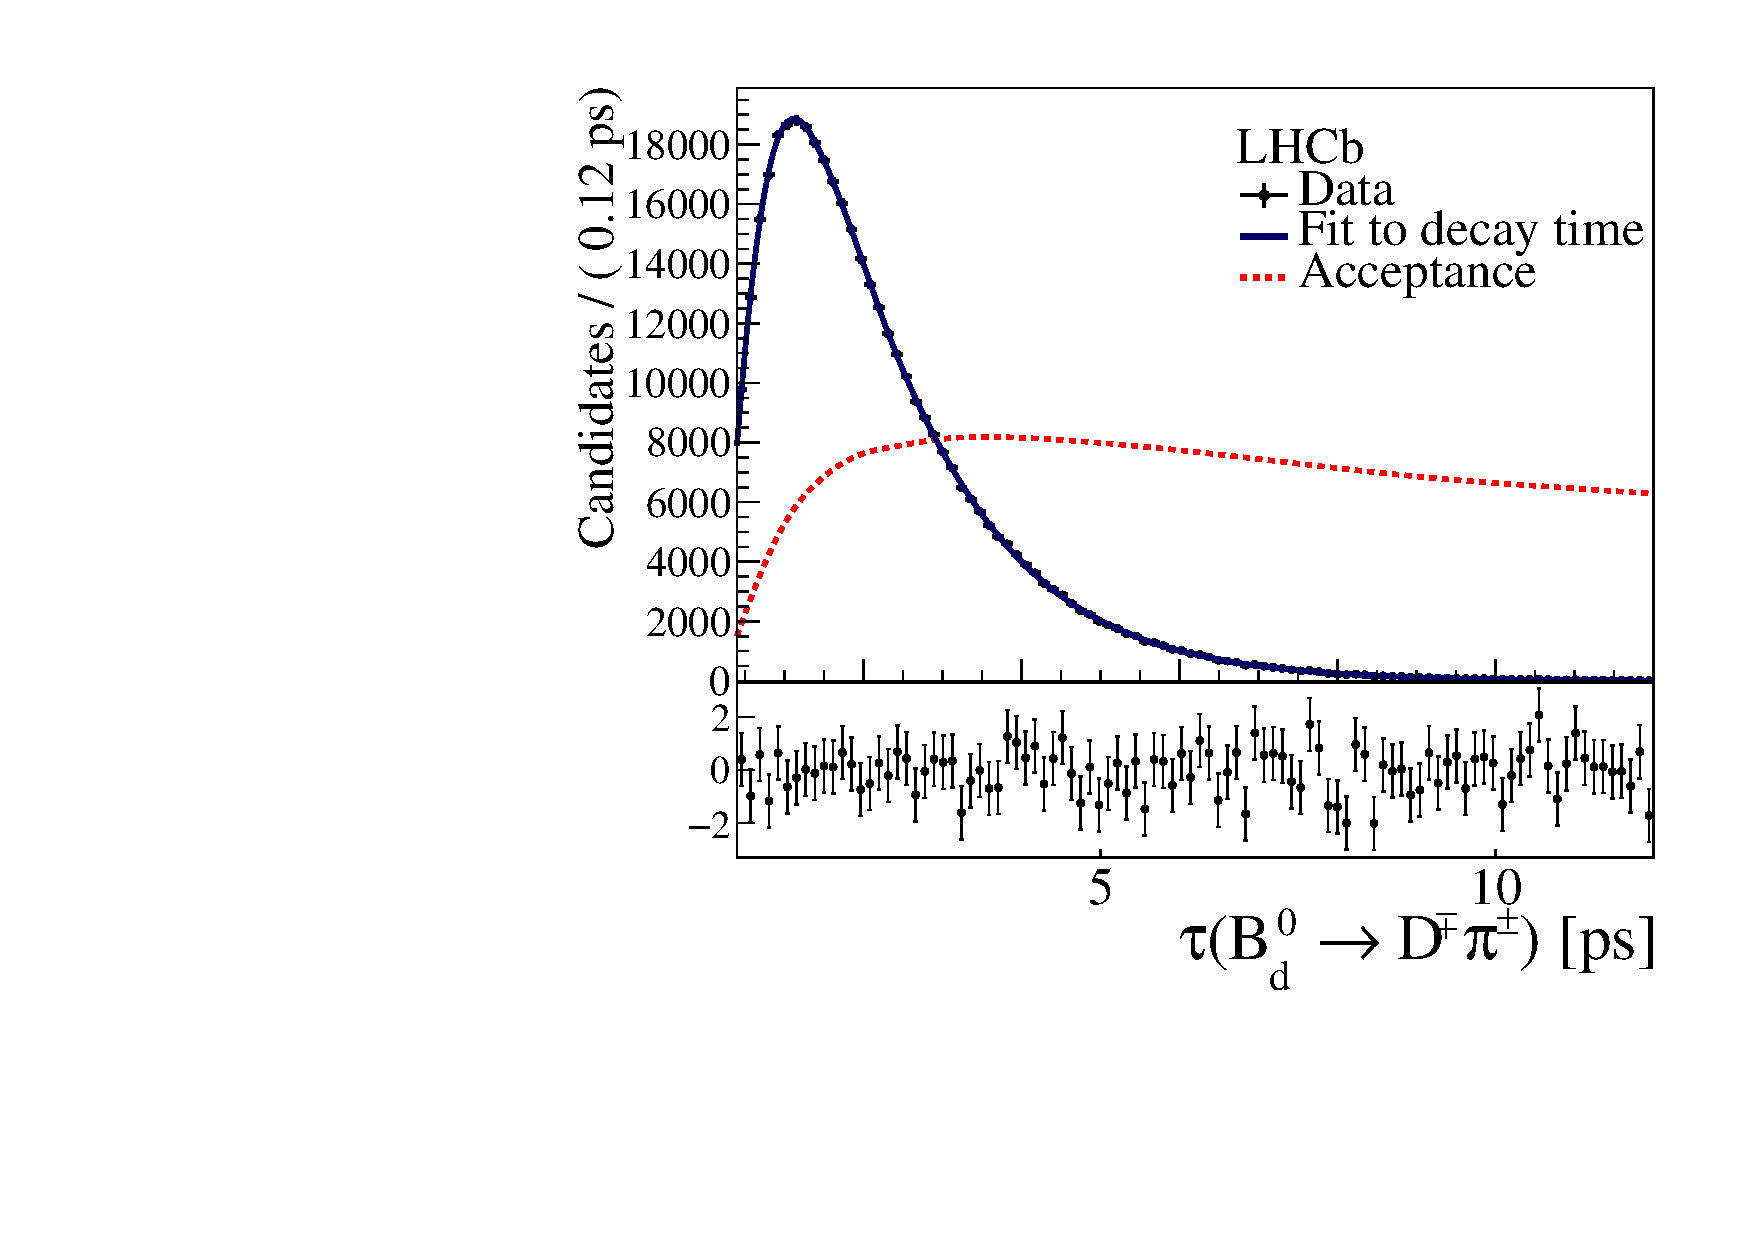
\includegraphics[width=0.49\linewidth]{05DecaytimeFit/figs/datafit/sFit_Bd2DPi.pdf}
                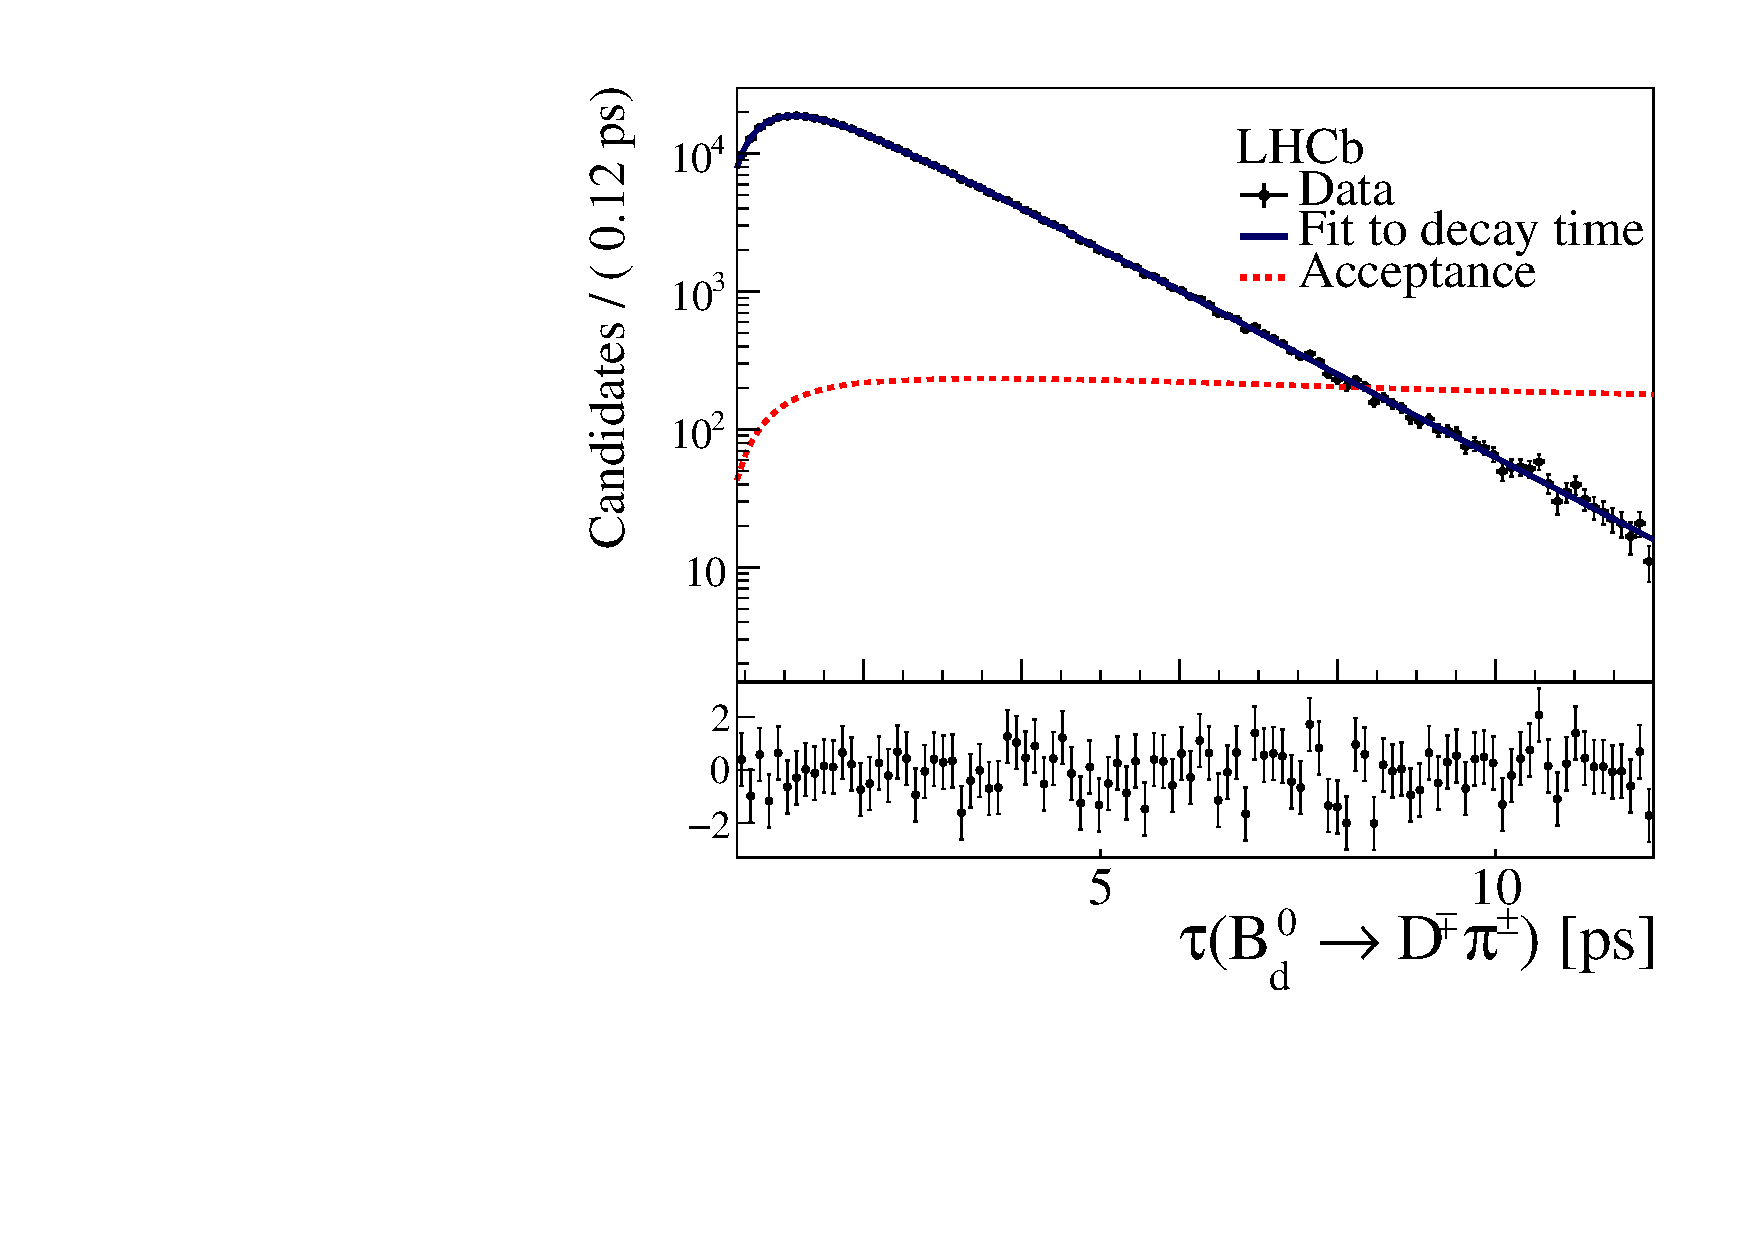
\includegraphics[width=0.49\linewidth]{05DecaytimeFit/figs/datafit/sFit_log_Bd2DPi.pdf}
	\end{center}
        \vspace{-4mm}
	\caption{Distribution of the reconstructed decay time of \emph{sWeighted} $\Bz\to\Dmp\pipm$ decays (data points), 
	with fit model superimposed (blue curve), and fitted acceptance function (red dotted curve), in linear (left) and logarithmic (right) scale.}
	\label{fig:timefitplot}
\end{figure}
\begin{figure}[htpb]
  \begin{center}
    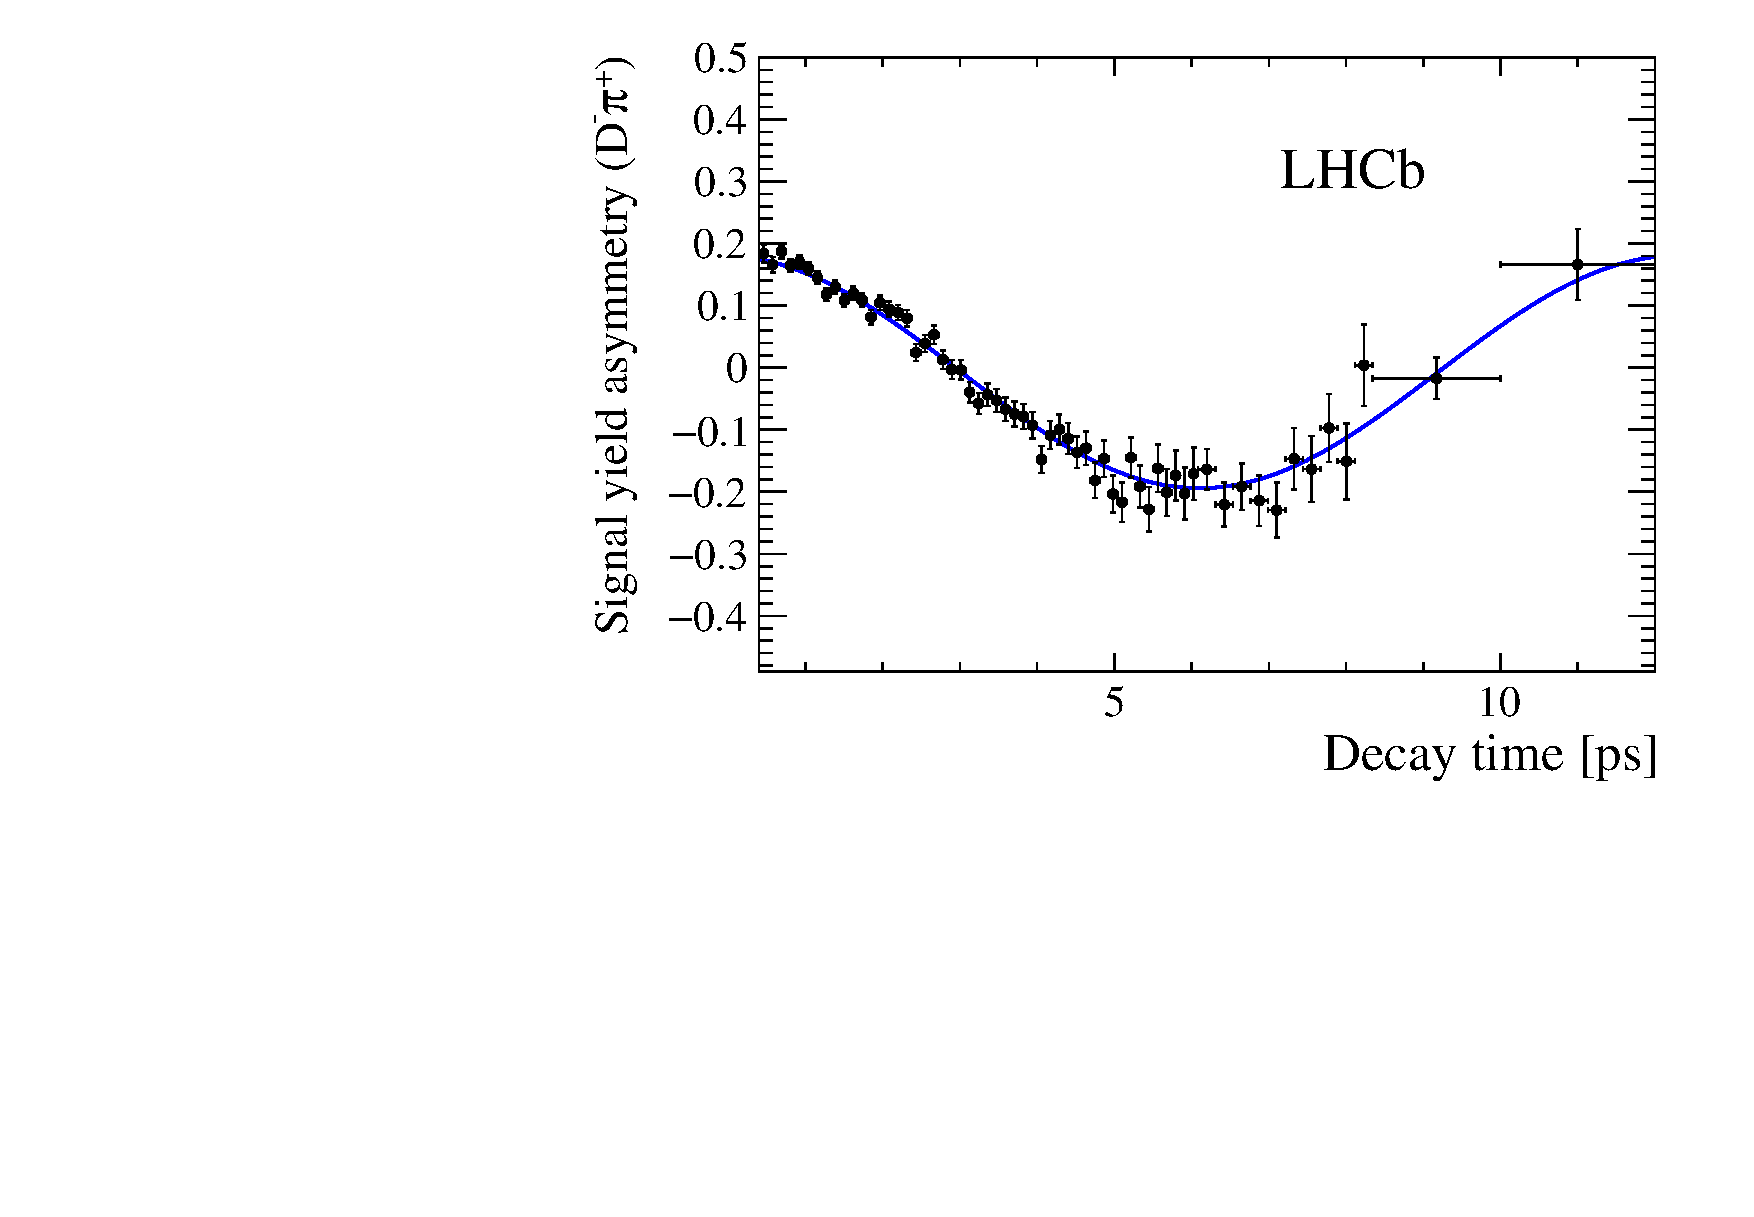
\includegraphics[width=0.49\linewidth]{05DecaytimeFit/figs/datafit/Asymmetry_f.pdf}
    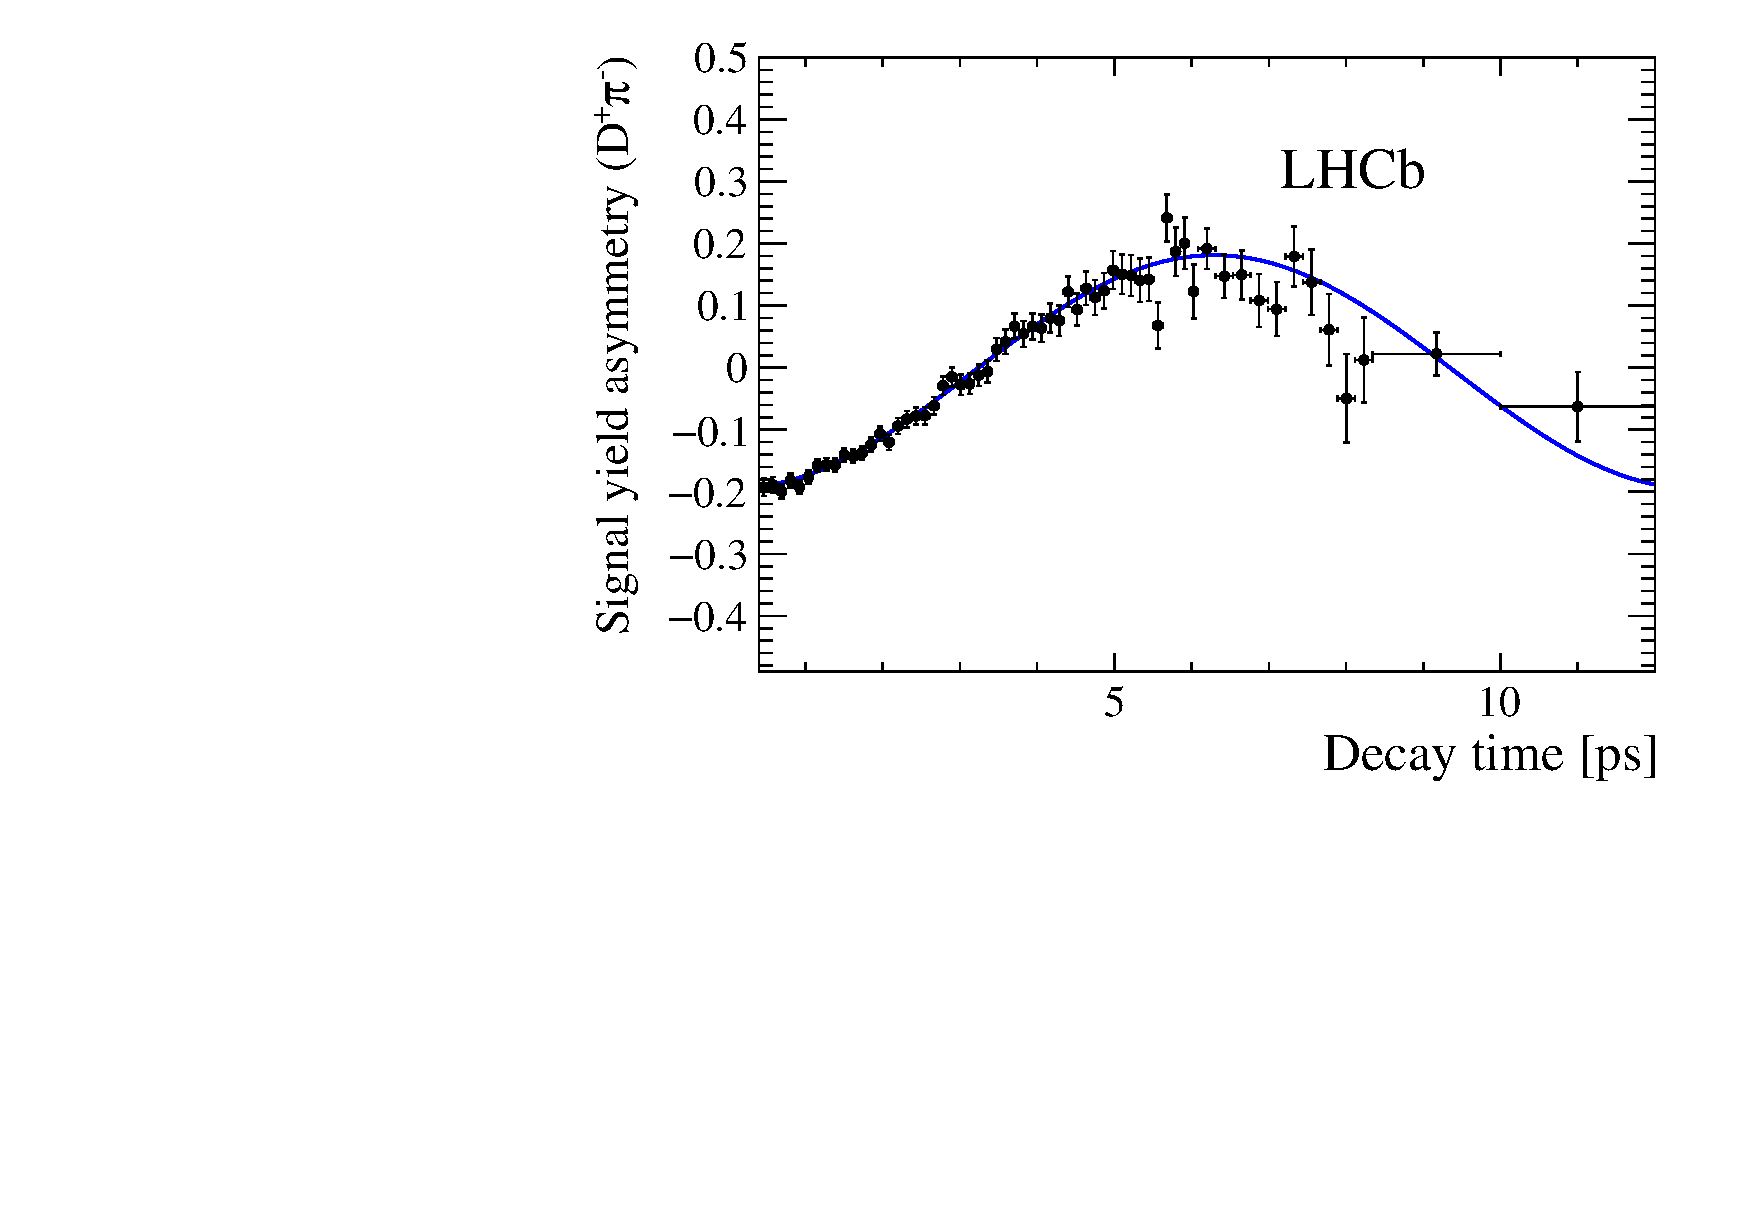
\includegraphics[width=0.49\linewidth]{05DecaytimeFit/figs/datafit/Asymmetry_fbar.pdf}
  \end{center}
  \vspace{-4mm}
  \caption{Time-dependent asymmetry between $\Bz$ and $\Bzb$ decays (data points) for the $\Dm\pip$ (left) and $\Dp\pim$ (right) final states, with fit model superimposed (blue curve).}
  \label{fig:asymplot}
\end{figure}
\begin{figure}[t]
  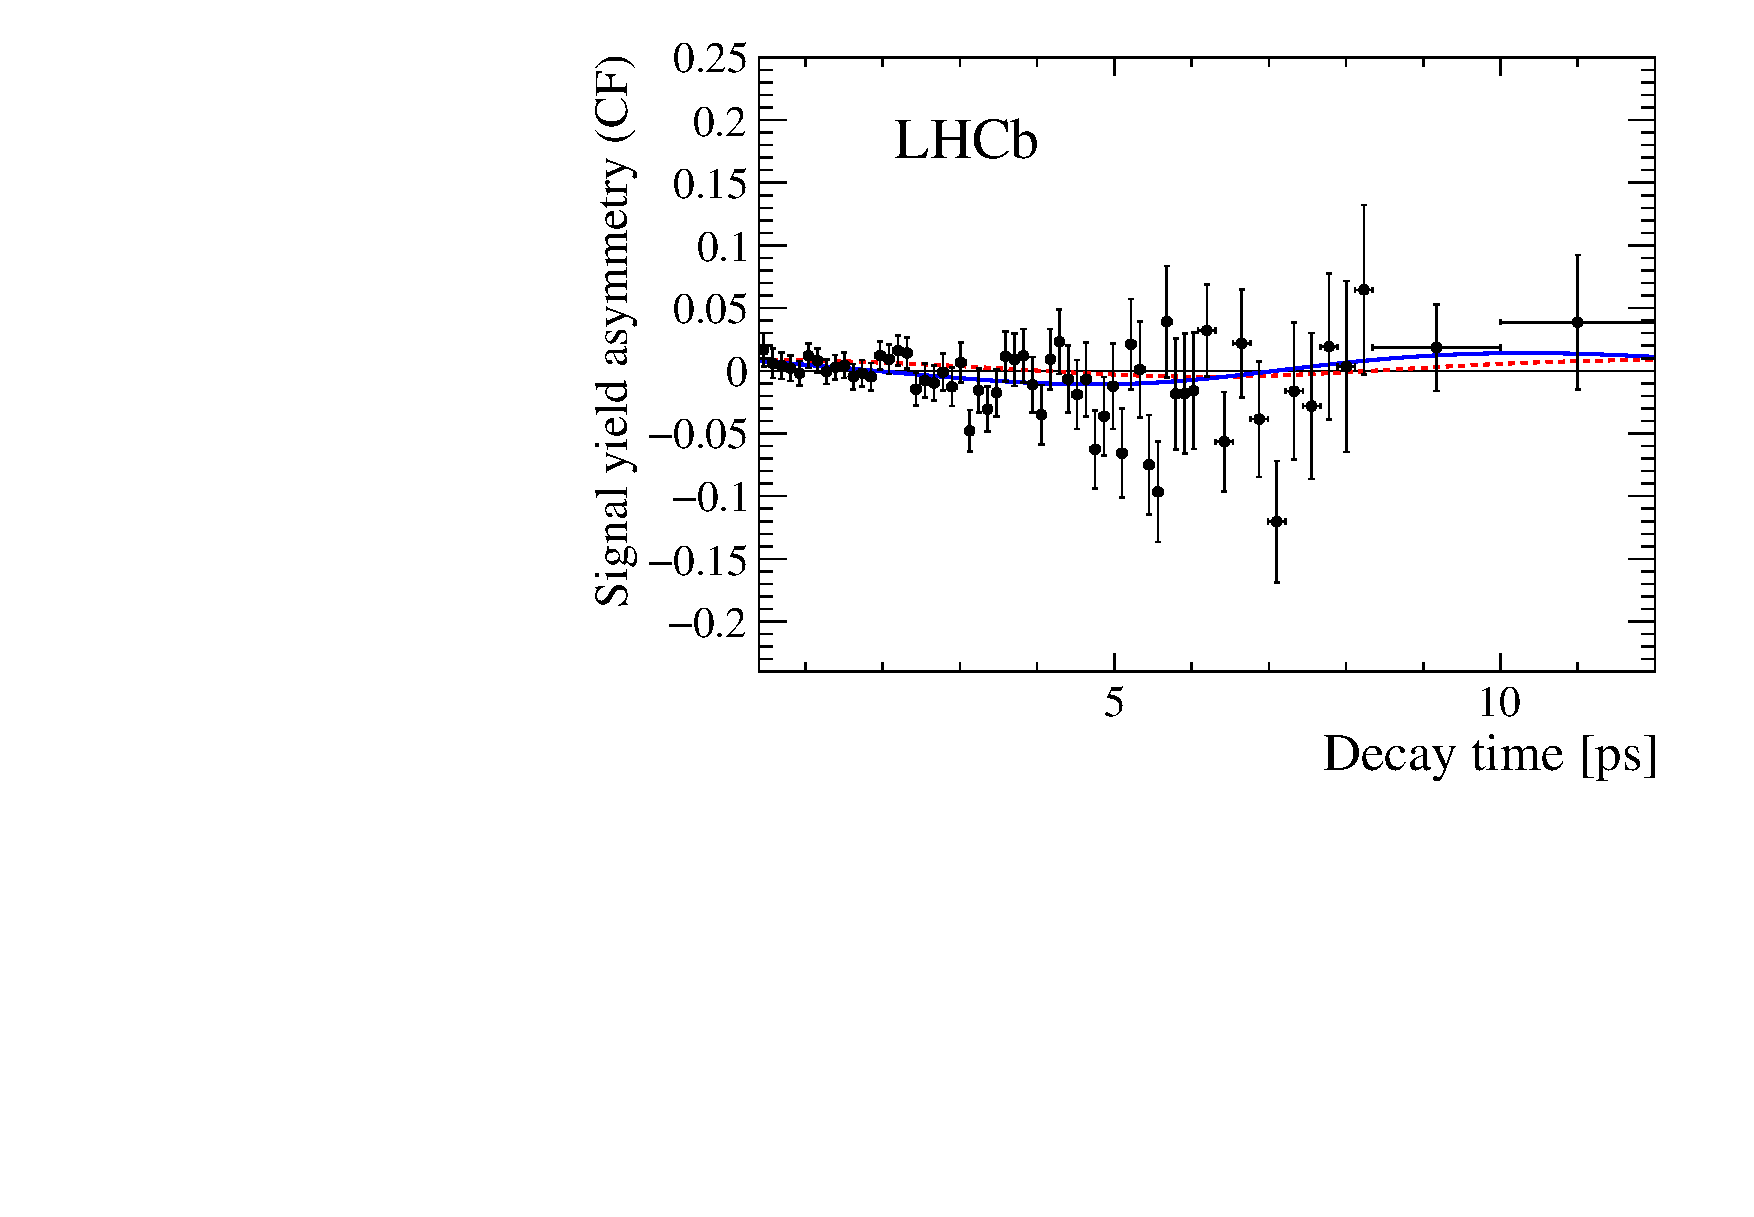
\includegraphics[width=0.45\textwidth]{05DecaytimeFit/figs/datafit/SAsymmetry_CF.pdf}
  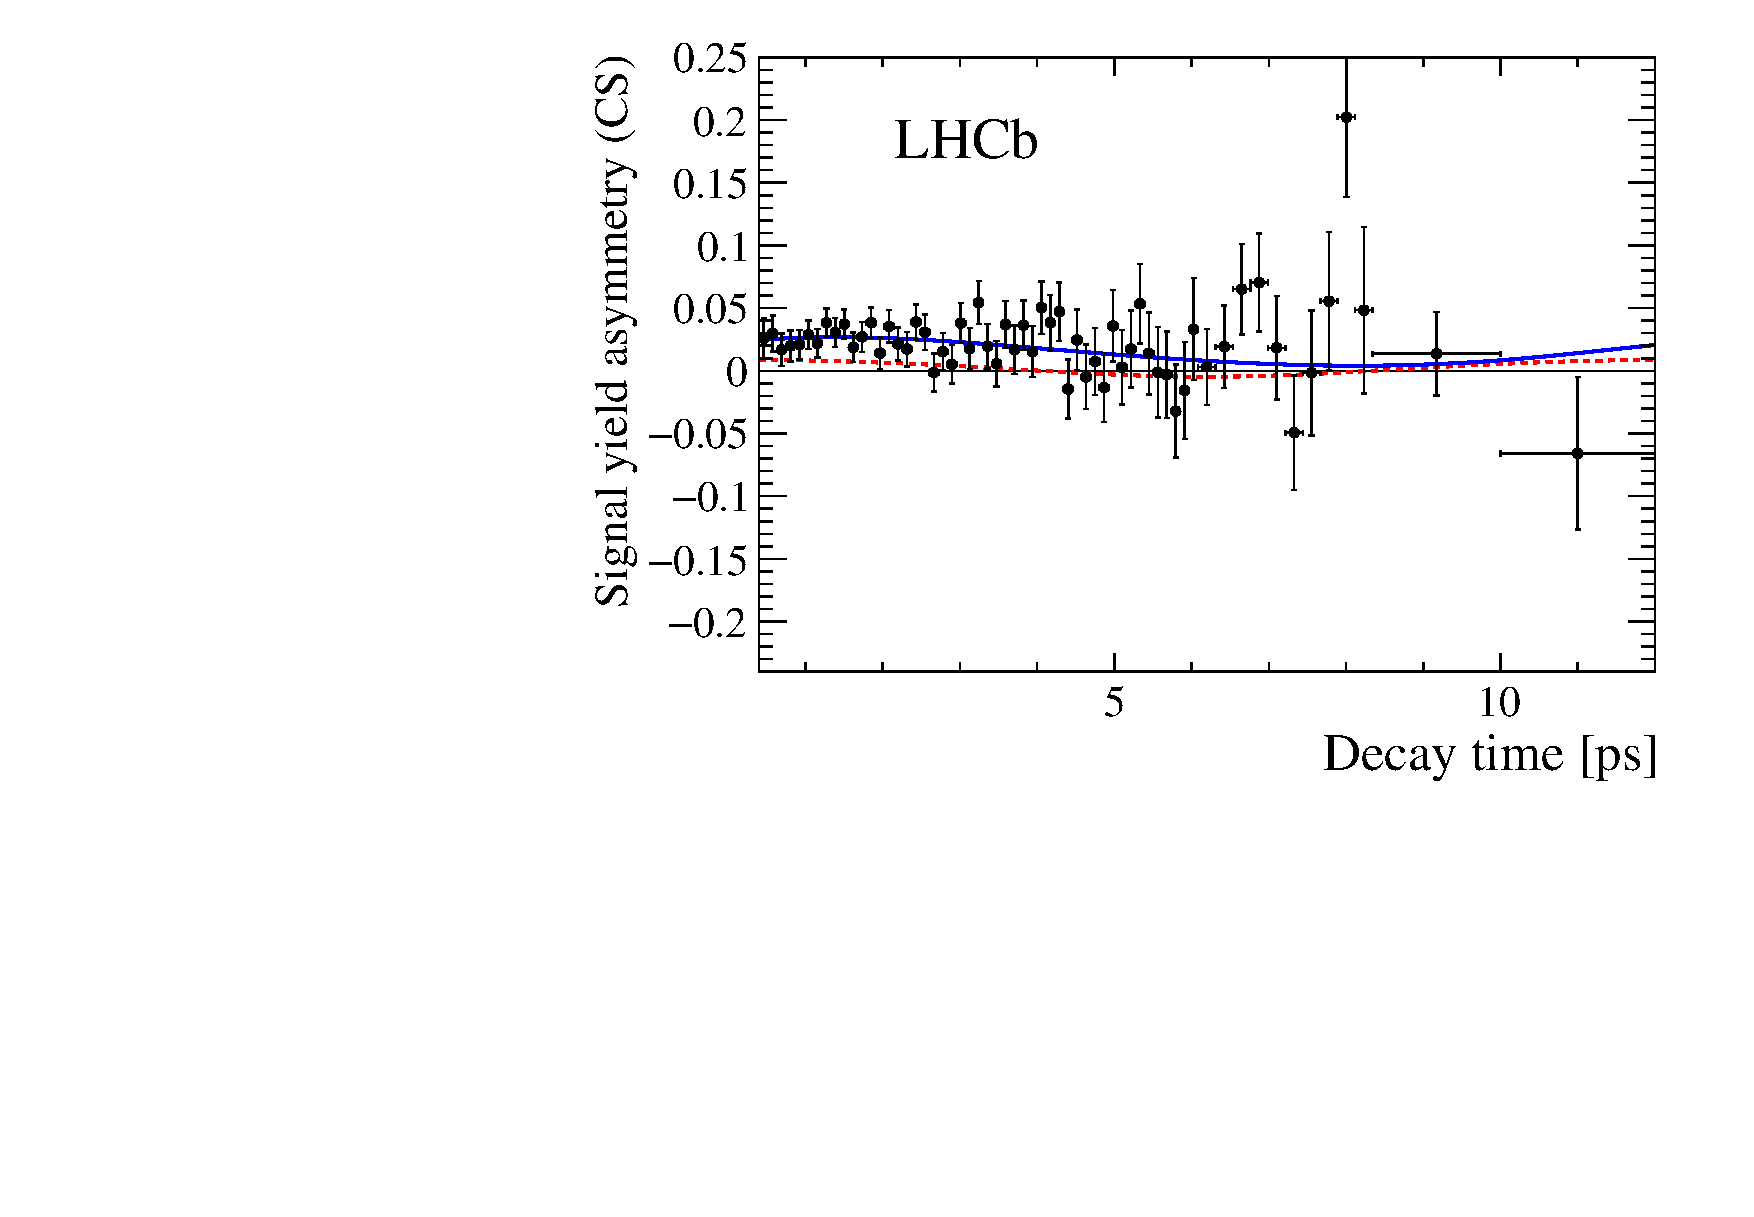
\includegraphics[width=0.45\textwidth]{05DecaytimeFit/figs/datafit/SAsymmetry_CS.pdf}
\vspace{-2mm}
\caption{\label{fig:asymmetries} Decay-time-dependent signal-yield asymmetries
for (left) Cabibbo-favoured and (right) Cabibbo-suppressed decay topologies, defined in Eq.~\ref{eq:CFSAsym}. 
The points with error bars are the data,
the blue solid curve is the fit model, and the red dotted curve indicates the fit model when
$\Sfb\equiv -\Sf$ (\ie~\CP~conservation in the interference between mixing and decay) is required.}
\end{figure}

\begin{figure}[t]
	\begin{center}
		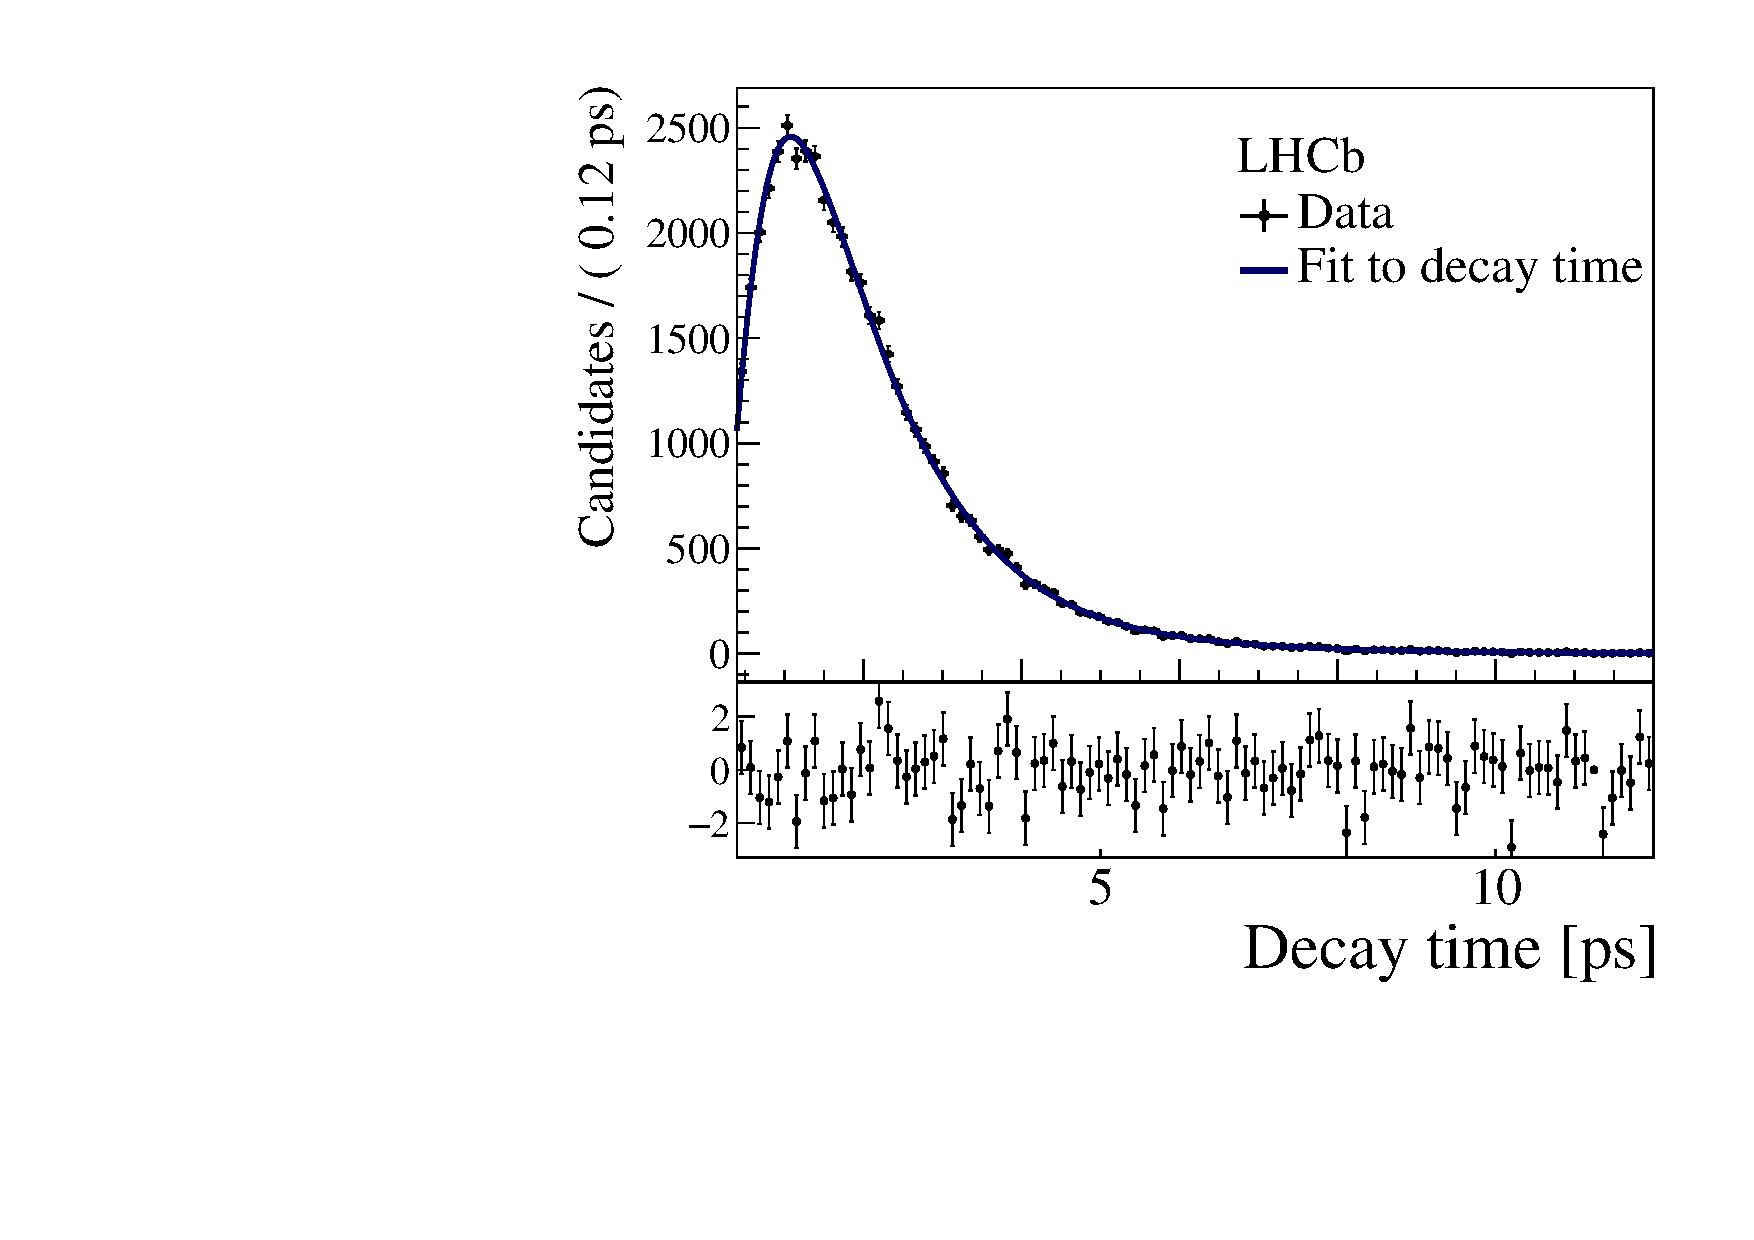
\includegraphics[width=0.4\linewidth]{05DecaytimeFit/figs/datafit/sFit_B2DmPipOSincl_Bd2DPi.pdf}
                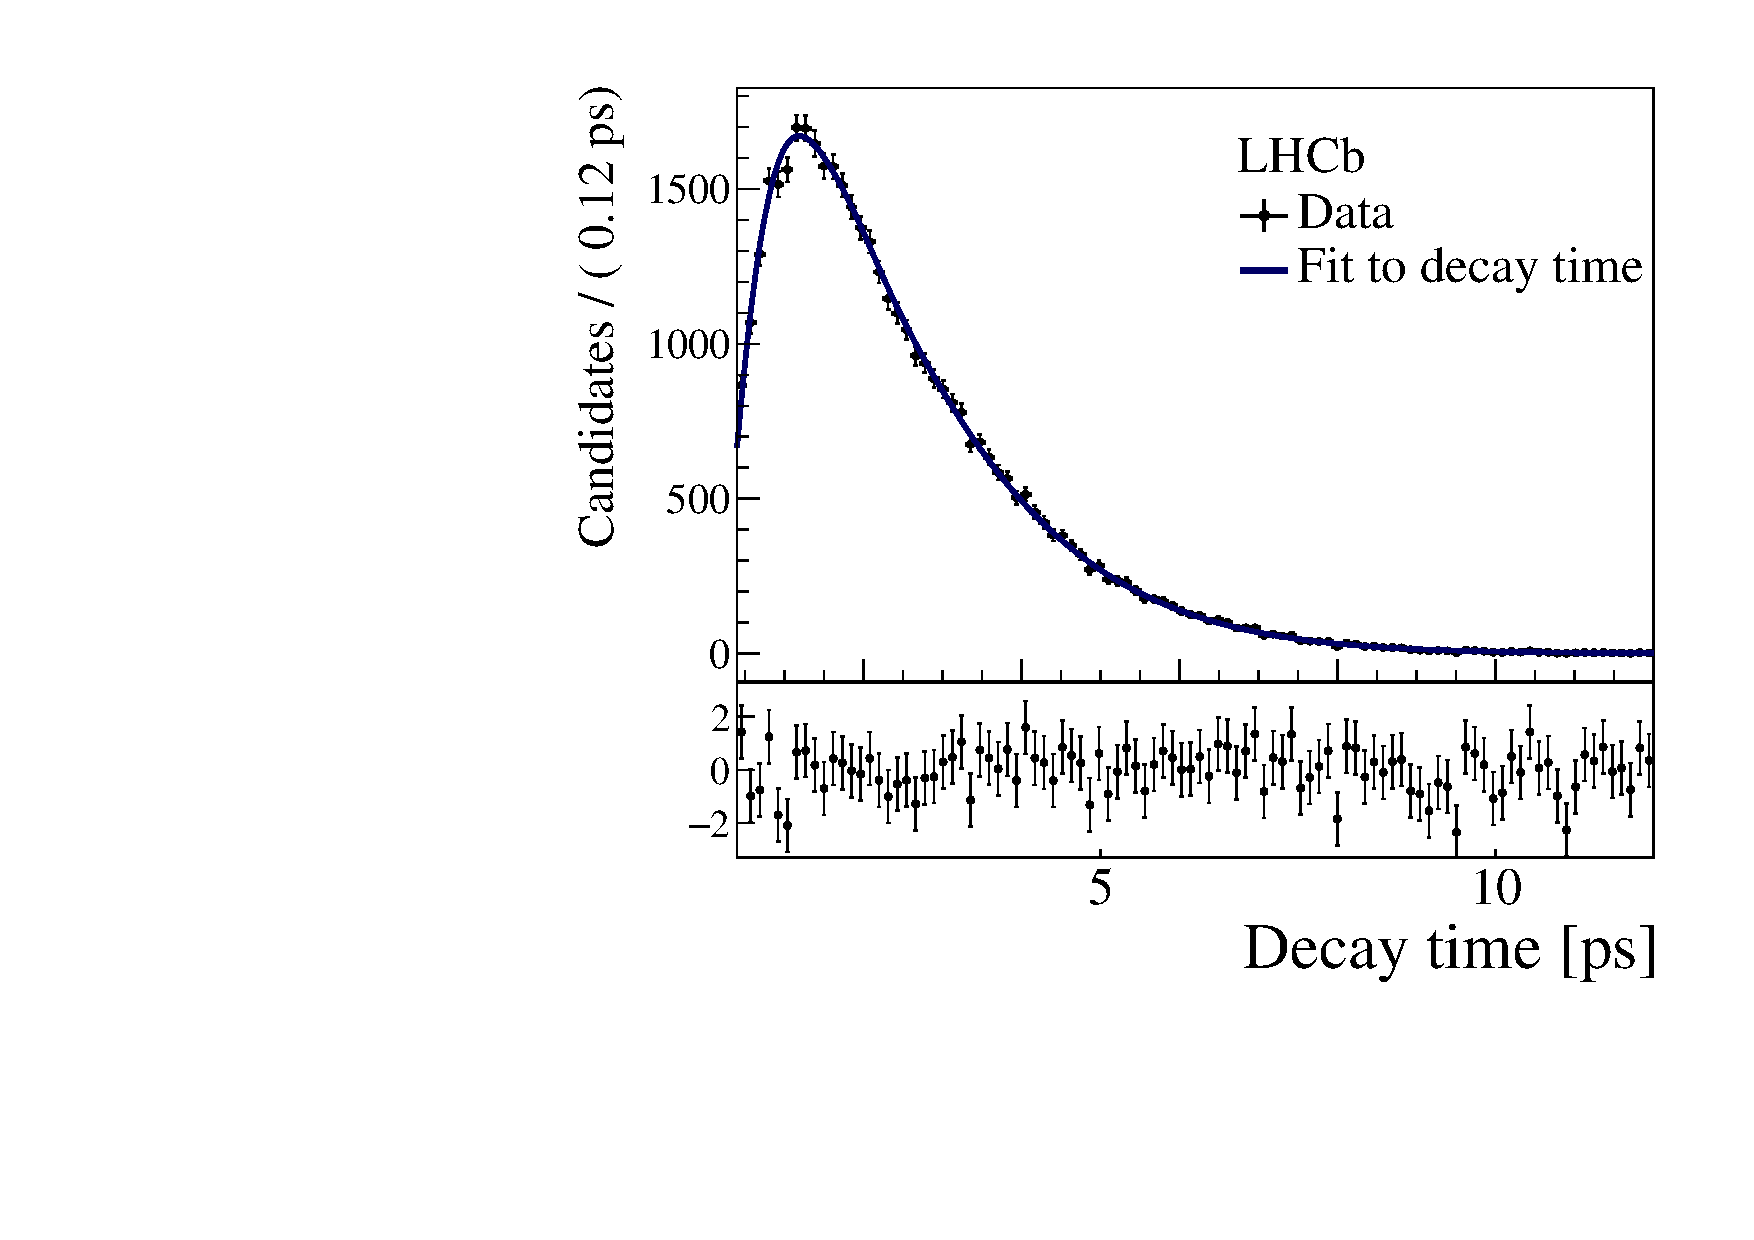
\includegraphics[width=0.4\linewidth]{05DecaytimeFit/figs/datafit/sFit_Bbar2DmPipOSincl_Bd2DPi.pdf}\\
                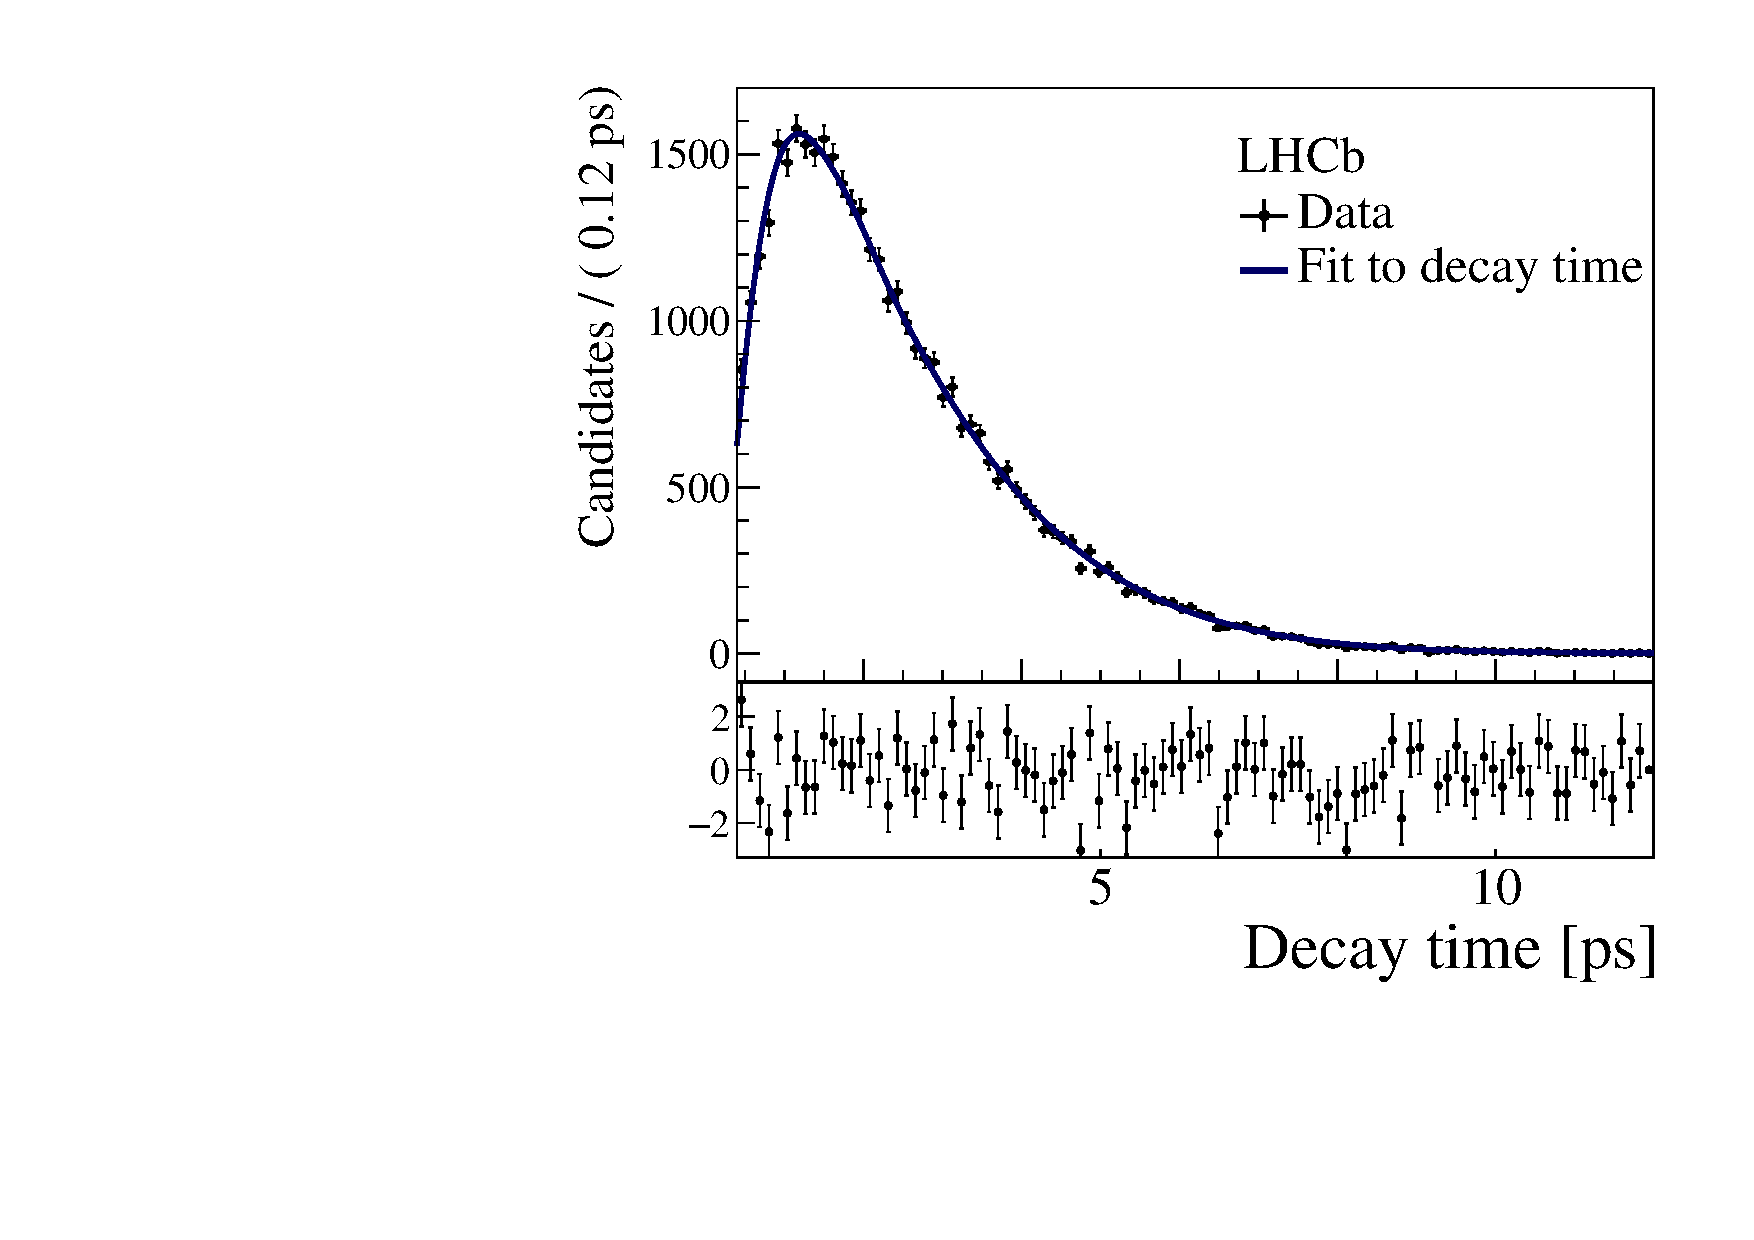
\includegraphics[width=0.4\linewidth]{05DecaytimeFit/figs/datafit/sFit_B2DpPimOSincl_Bd2DPi.pdf}
                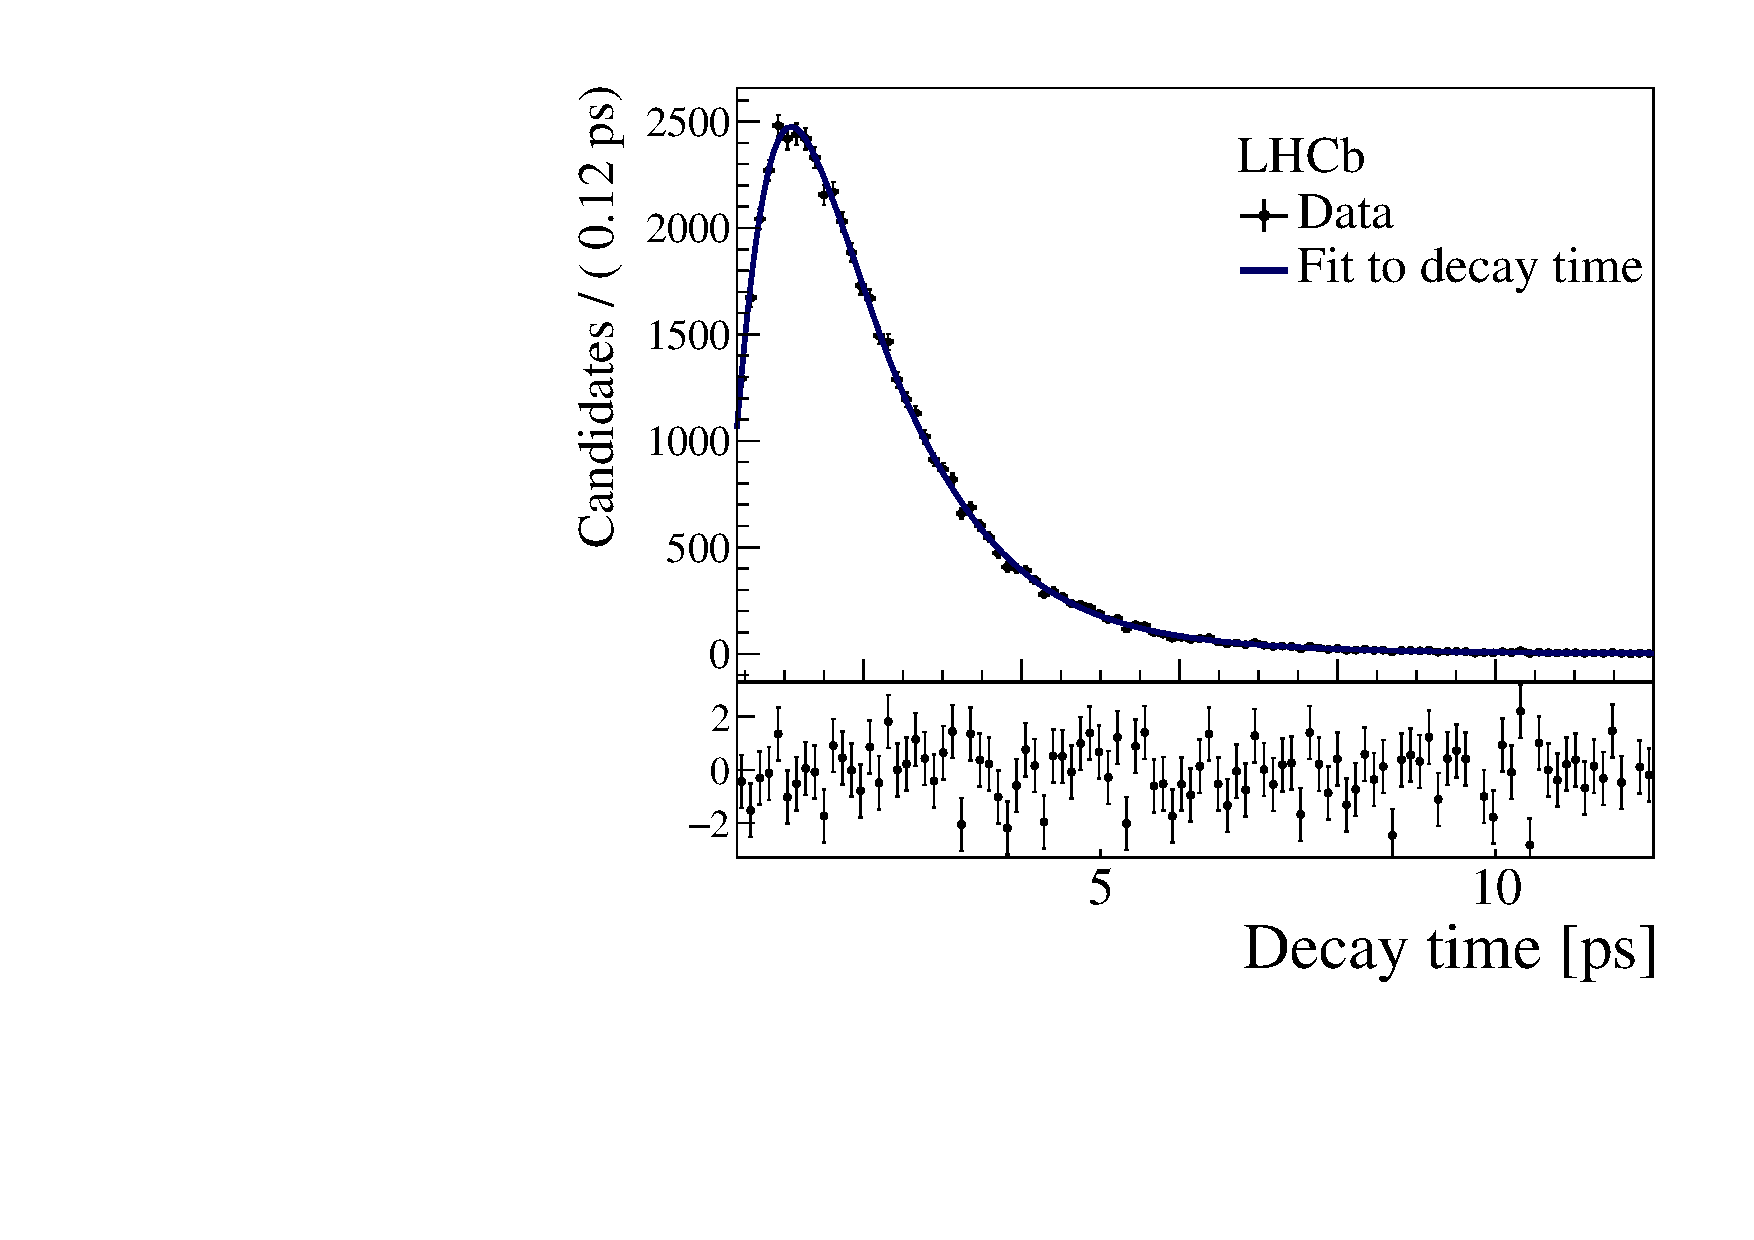
\includegraphics[width=0.4\linewidth]{05DecaytimeFit/figs/datafit/sFit_Bbar2DpPimOSincl_Bd2DPi.pdf}
	\end{center}
        \vspace{-2mm}
	\caption{Decay-time distributions of the \emph{sWeighted} data
  samples for (top left) $\Bz \to \Dm\pip$,  (top right) $\Bzb \to \Dm\pip$,  (bottom left) $\Bz \to \Dp\pim$
  and  (bottom right) $\Bzb \to \Dp\pim$ for OS inclusively tagged candidates. The fit result is superimposed as the blue curves.}
	\label{fig:timefitplot-4ratesOS}
\end{figure}

\begin{figure}[t]
        \begin{center}
                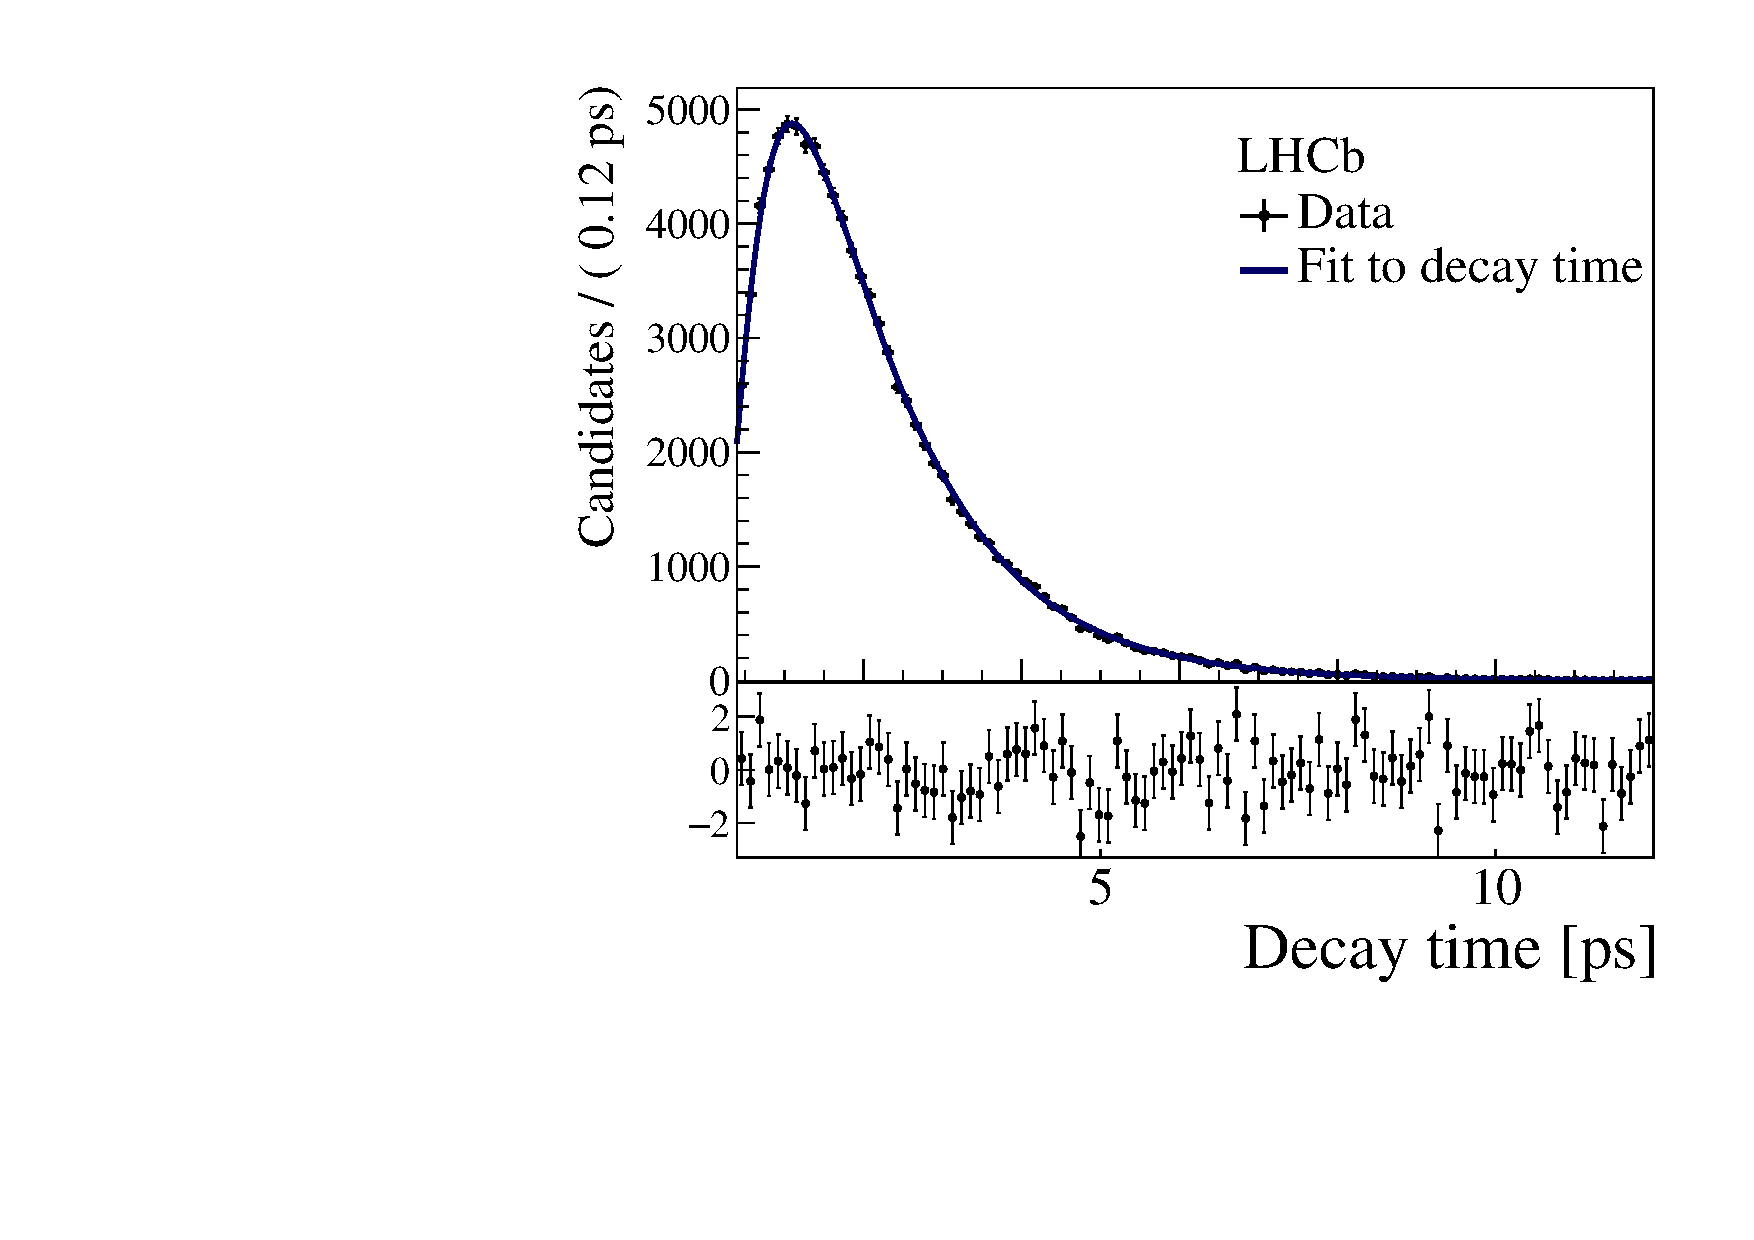
\includegraphics[width=0.4\linewidth]{05DecaytimeFit/figs/datafit/sFit_B2DmPipSSincl_Bd2DPi.pdf}
                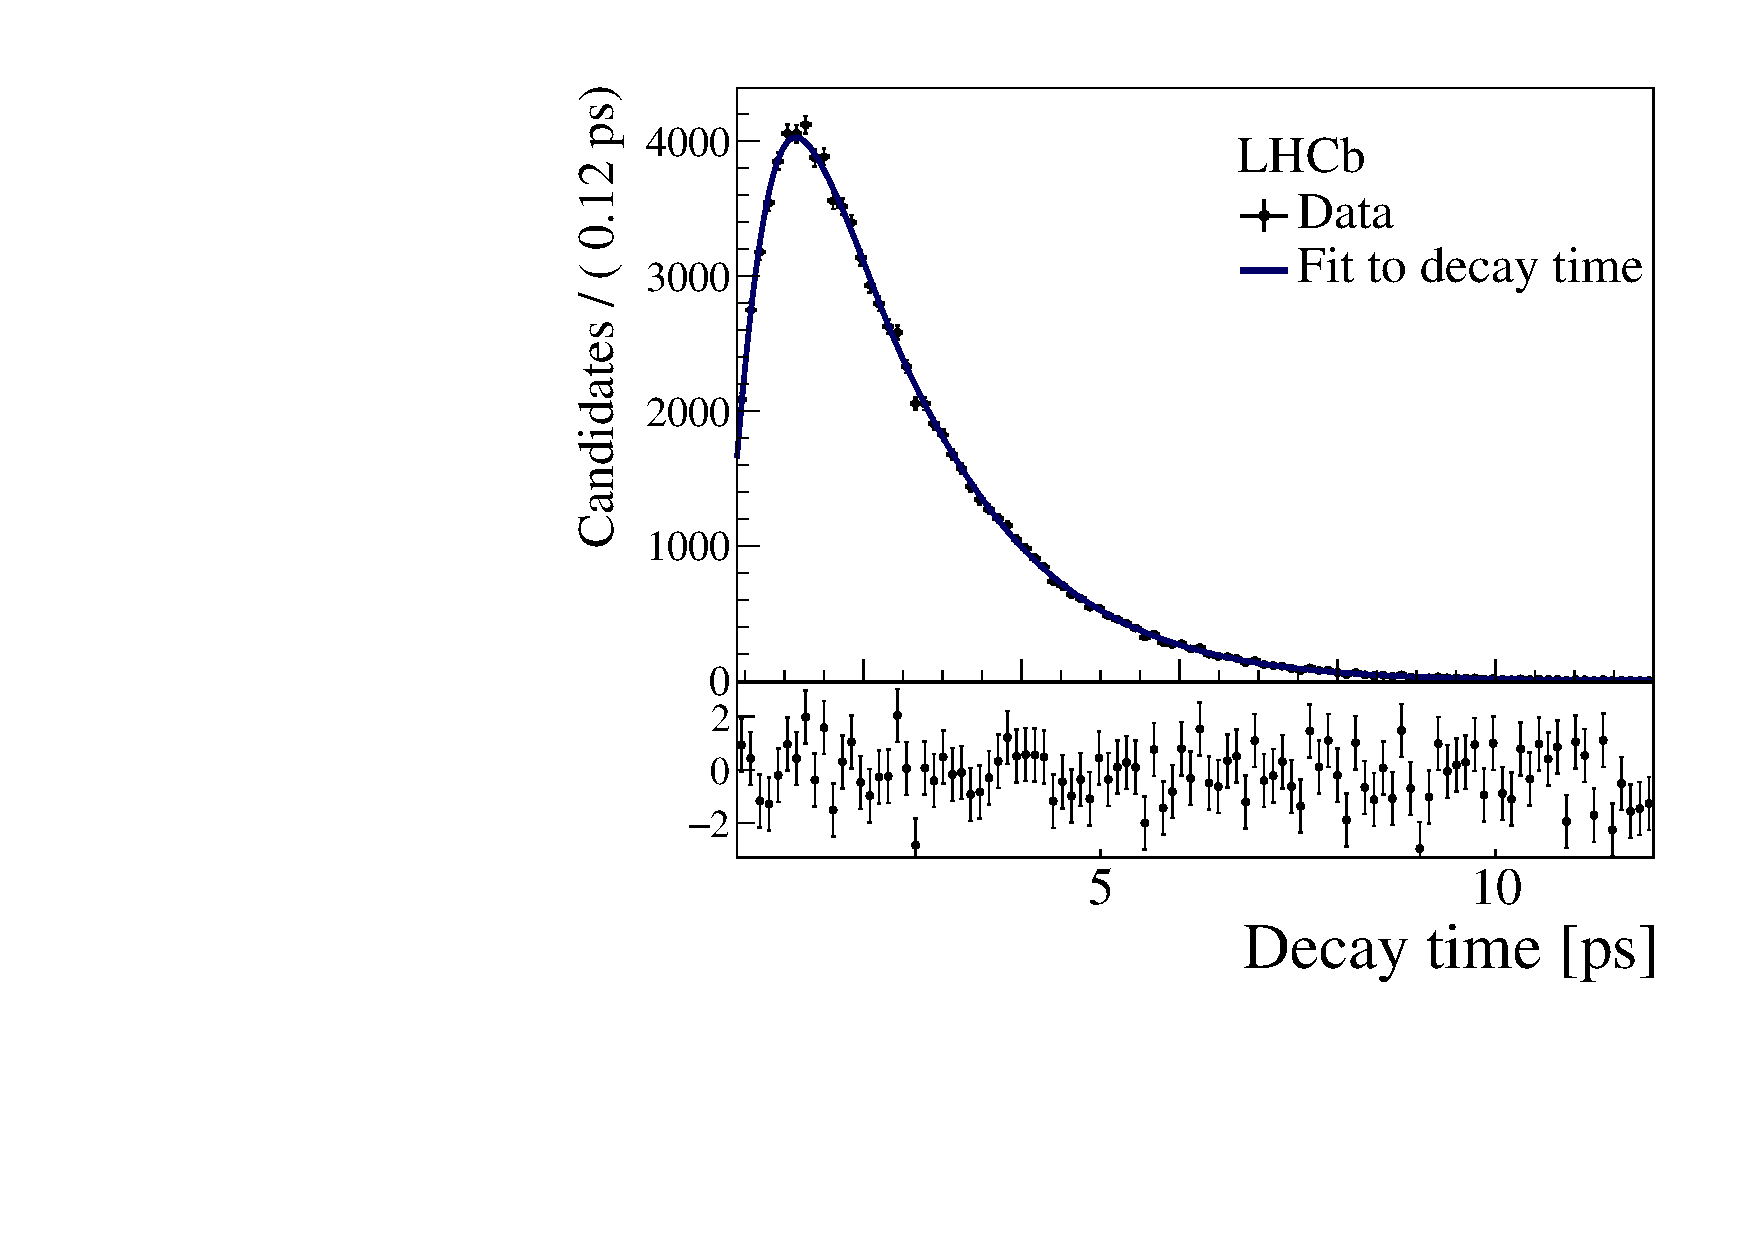
\includegraphics[width=0.4\linewidth]{05DecaytimeFit/figs/datafit/sFit_Bbar2DmPipSSincl_Bd2DPi.pdf}\\
                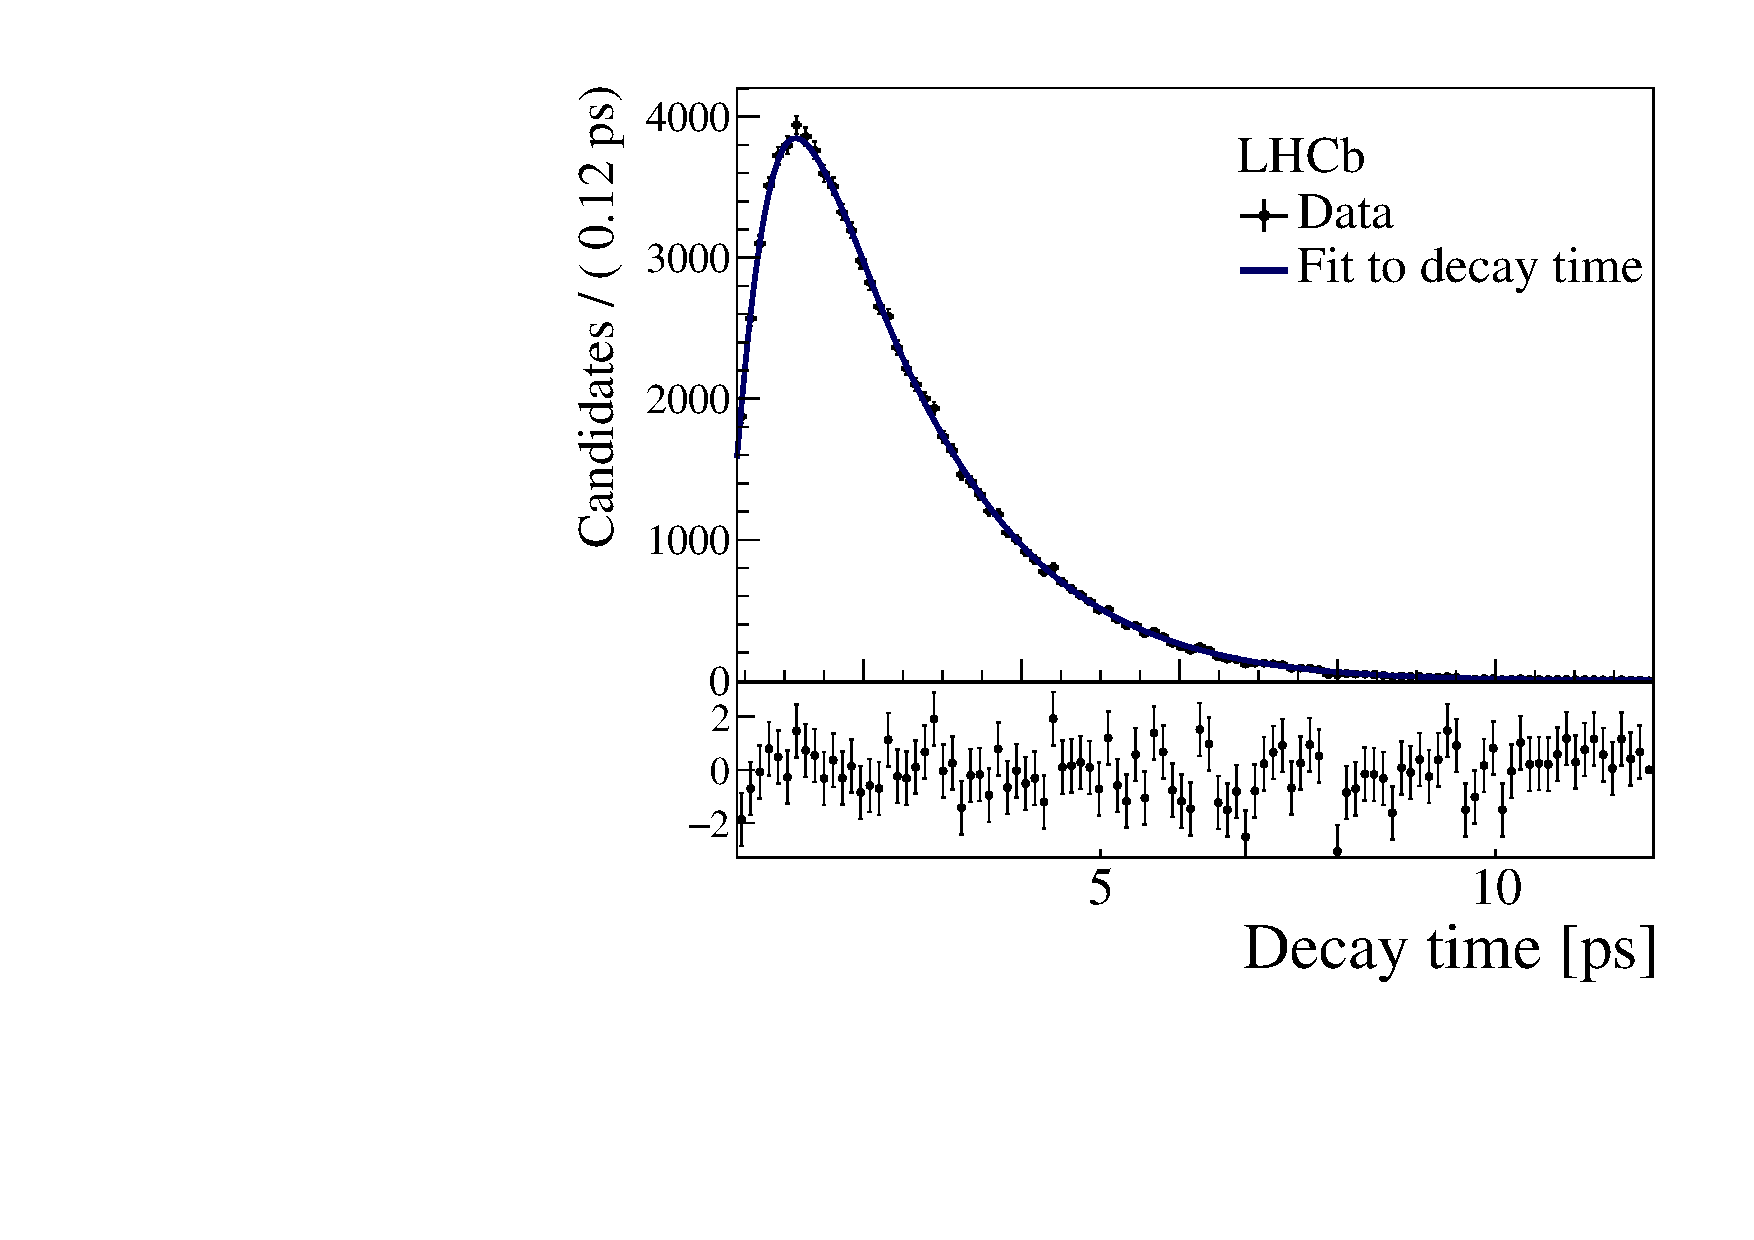
\includegraphics[width=0.4\linewidth]{05DecaytimeFit/figs/datafit/sFit_B2DpPimSSincl_Bd2DPi.pdf}
                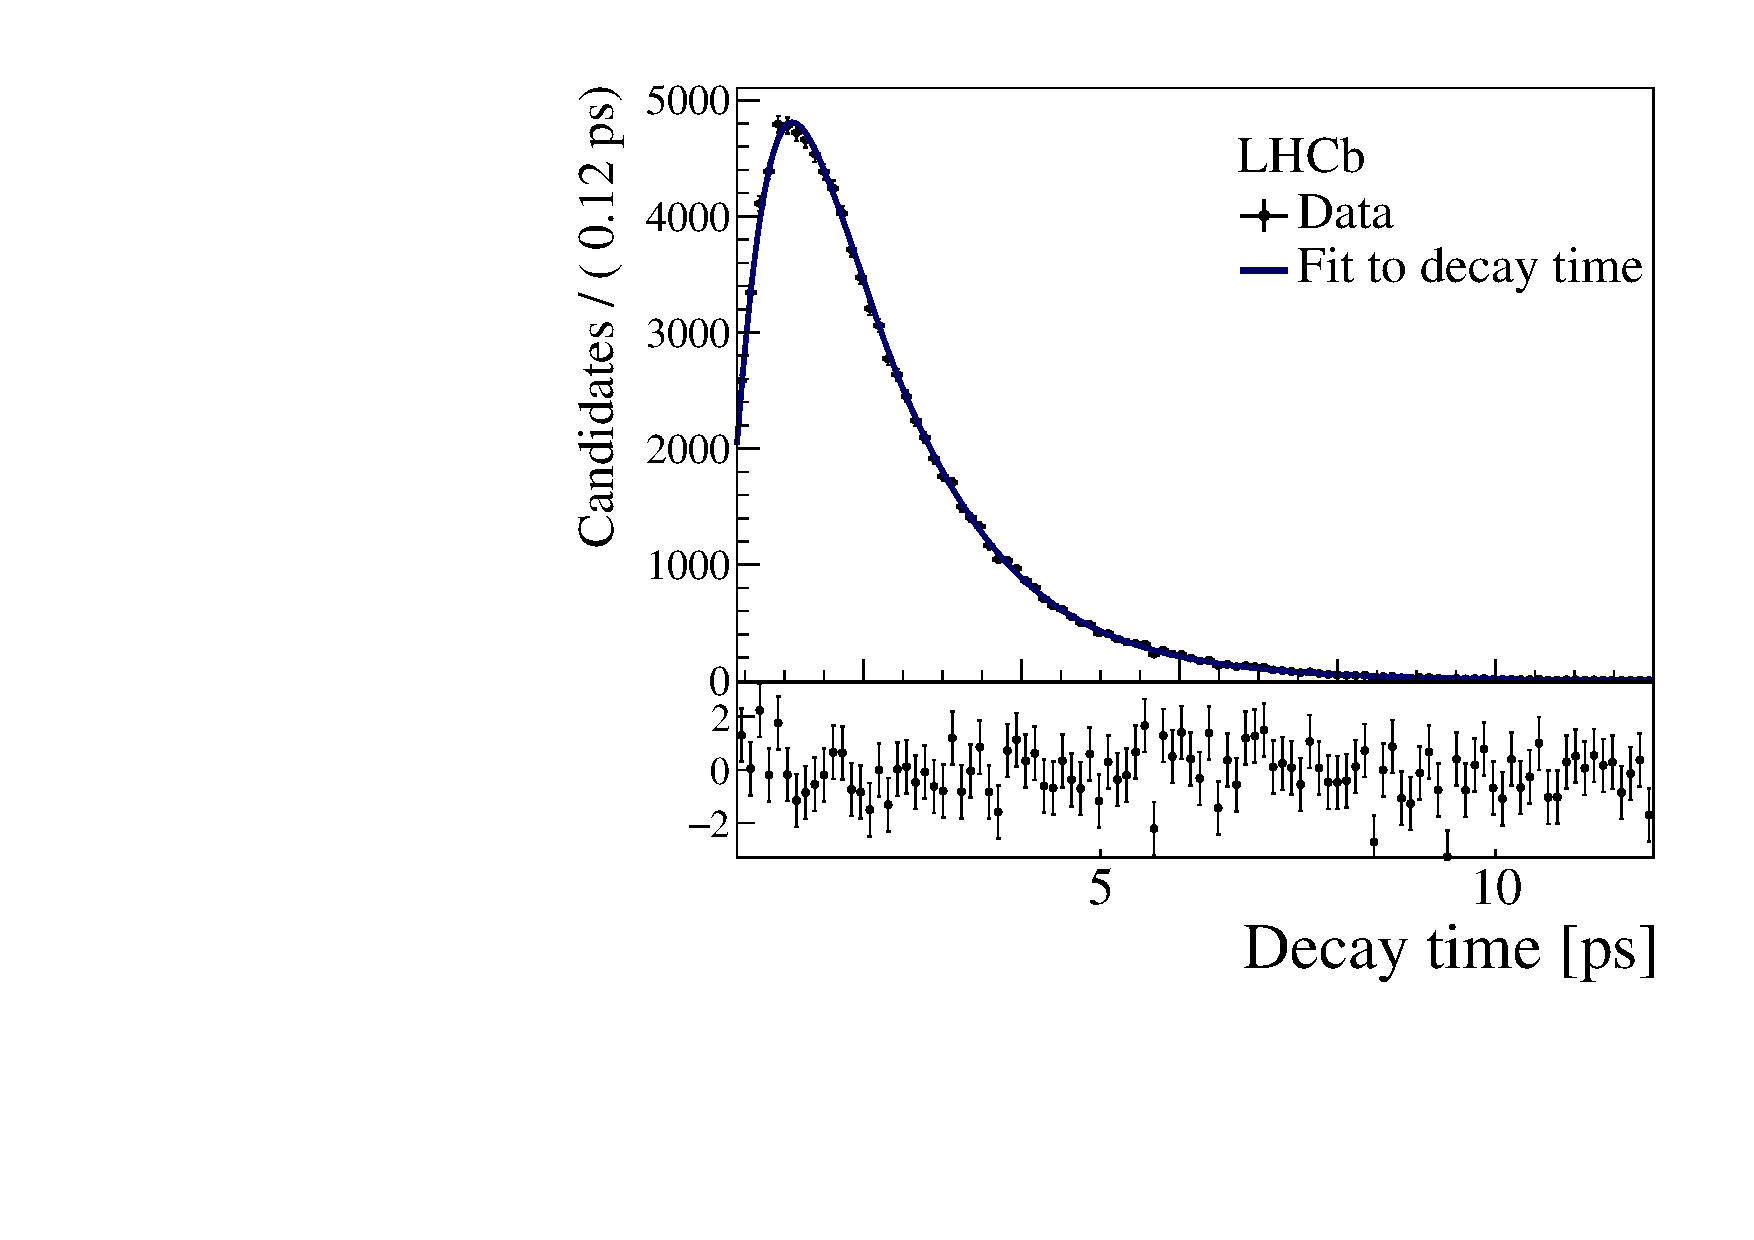
\includegraphics[width=0.4\linewidth]{05DecaytimeFit/figs/datafit/sFit_Bbar2DpPimSSincl_Bd2DPi.pdf}
        \end{center}
        \vspace{-2mm}
        \caption{Decay-time distributions of the \emph{sWeighted} data
  sample for (top left) $\Bz \to \Dm\pip$,  (top right) $\Bzb \to \Dm\pip$,  (bottom left) $\Bz \to \Dp\pim$
  and  (bottom right) $\Bzb \to \Dp\pim$ for SS inclusively tagged candidates. The fit result is superimposed as the blue curves.}
        \label{fig:timefitplot-4ratesSS}
\end{figure}

\begin{figure}[t]
        \begin{center}
            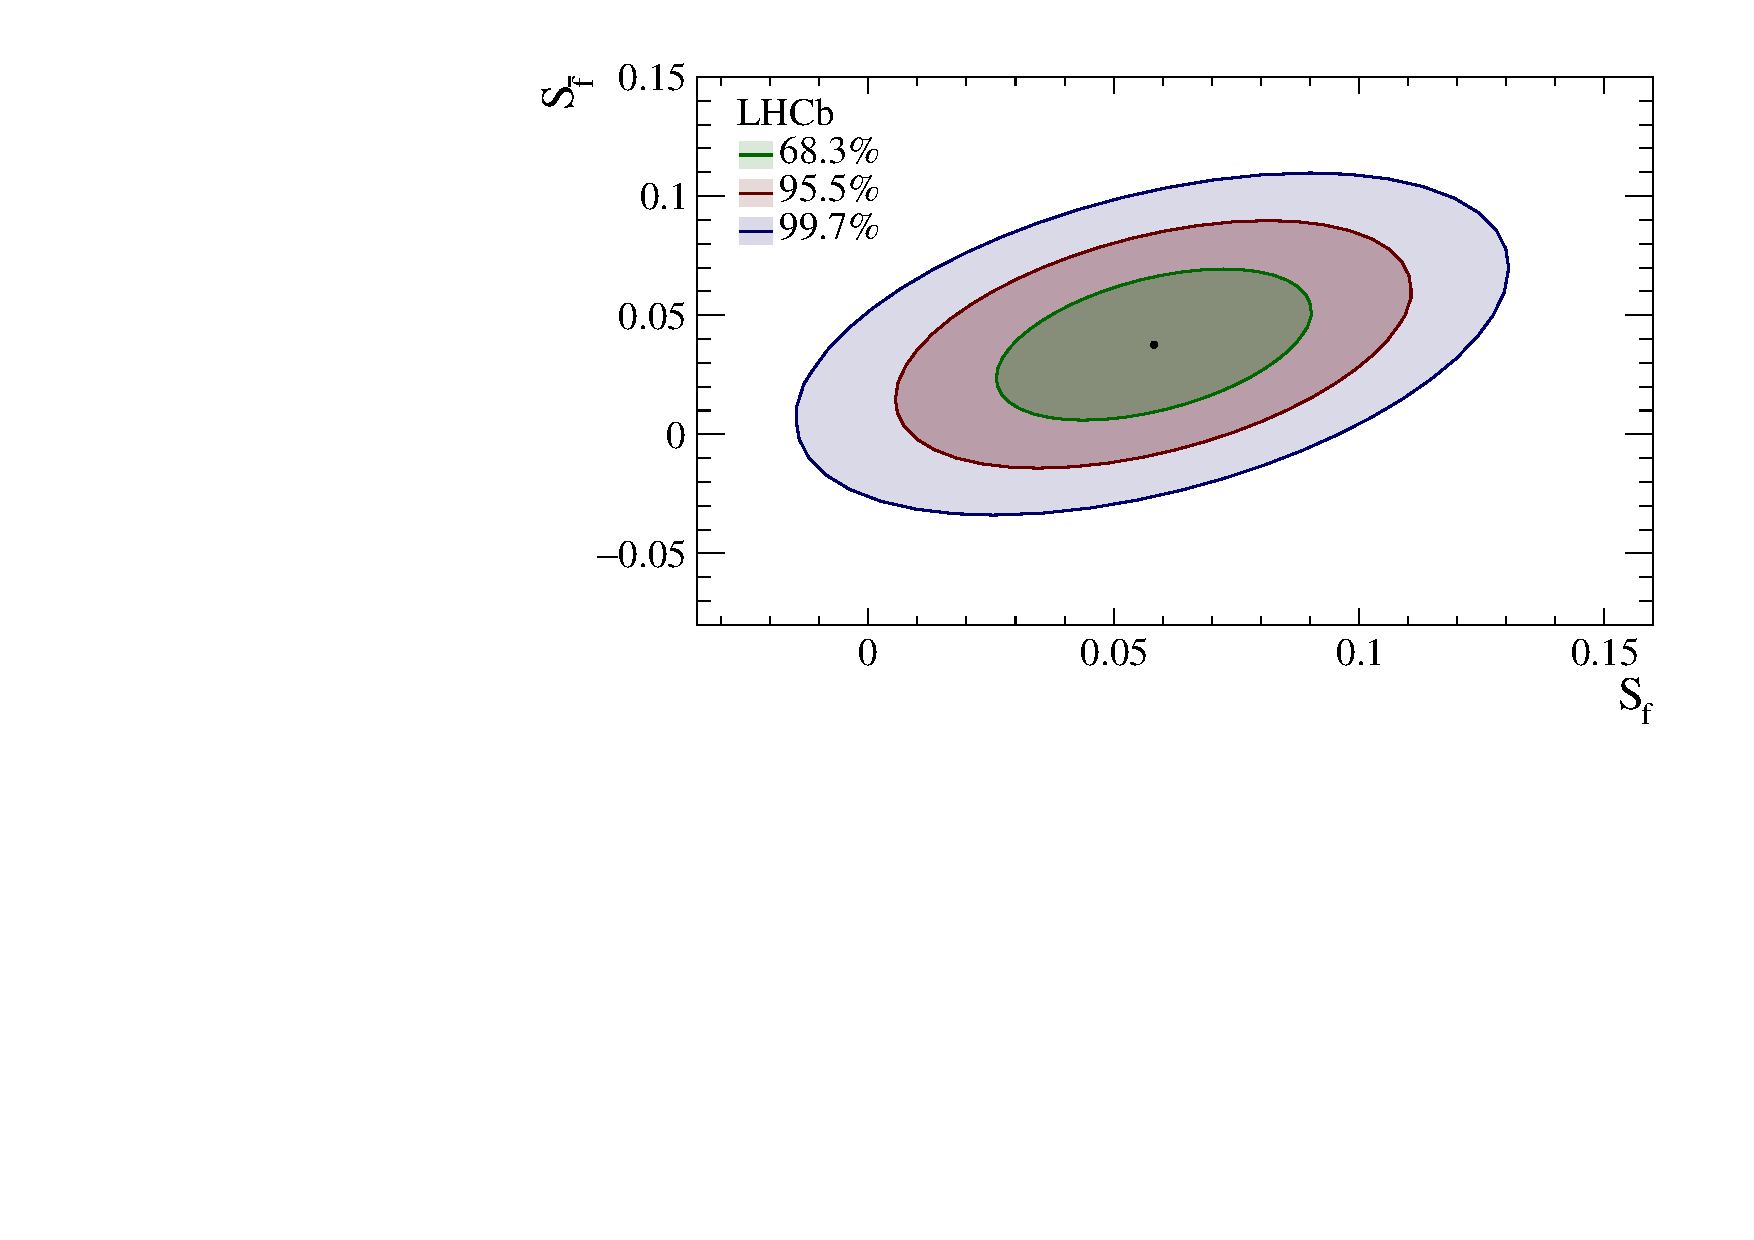
\includegraphics[width=0.48\linewidth]{05DecaytimeFit/figs/datafit/SfvsSfbar.pdf}
            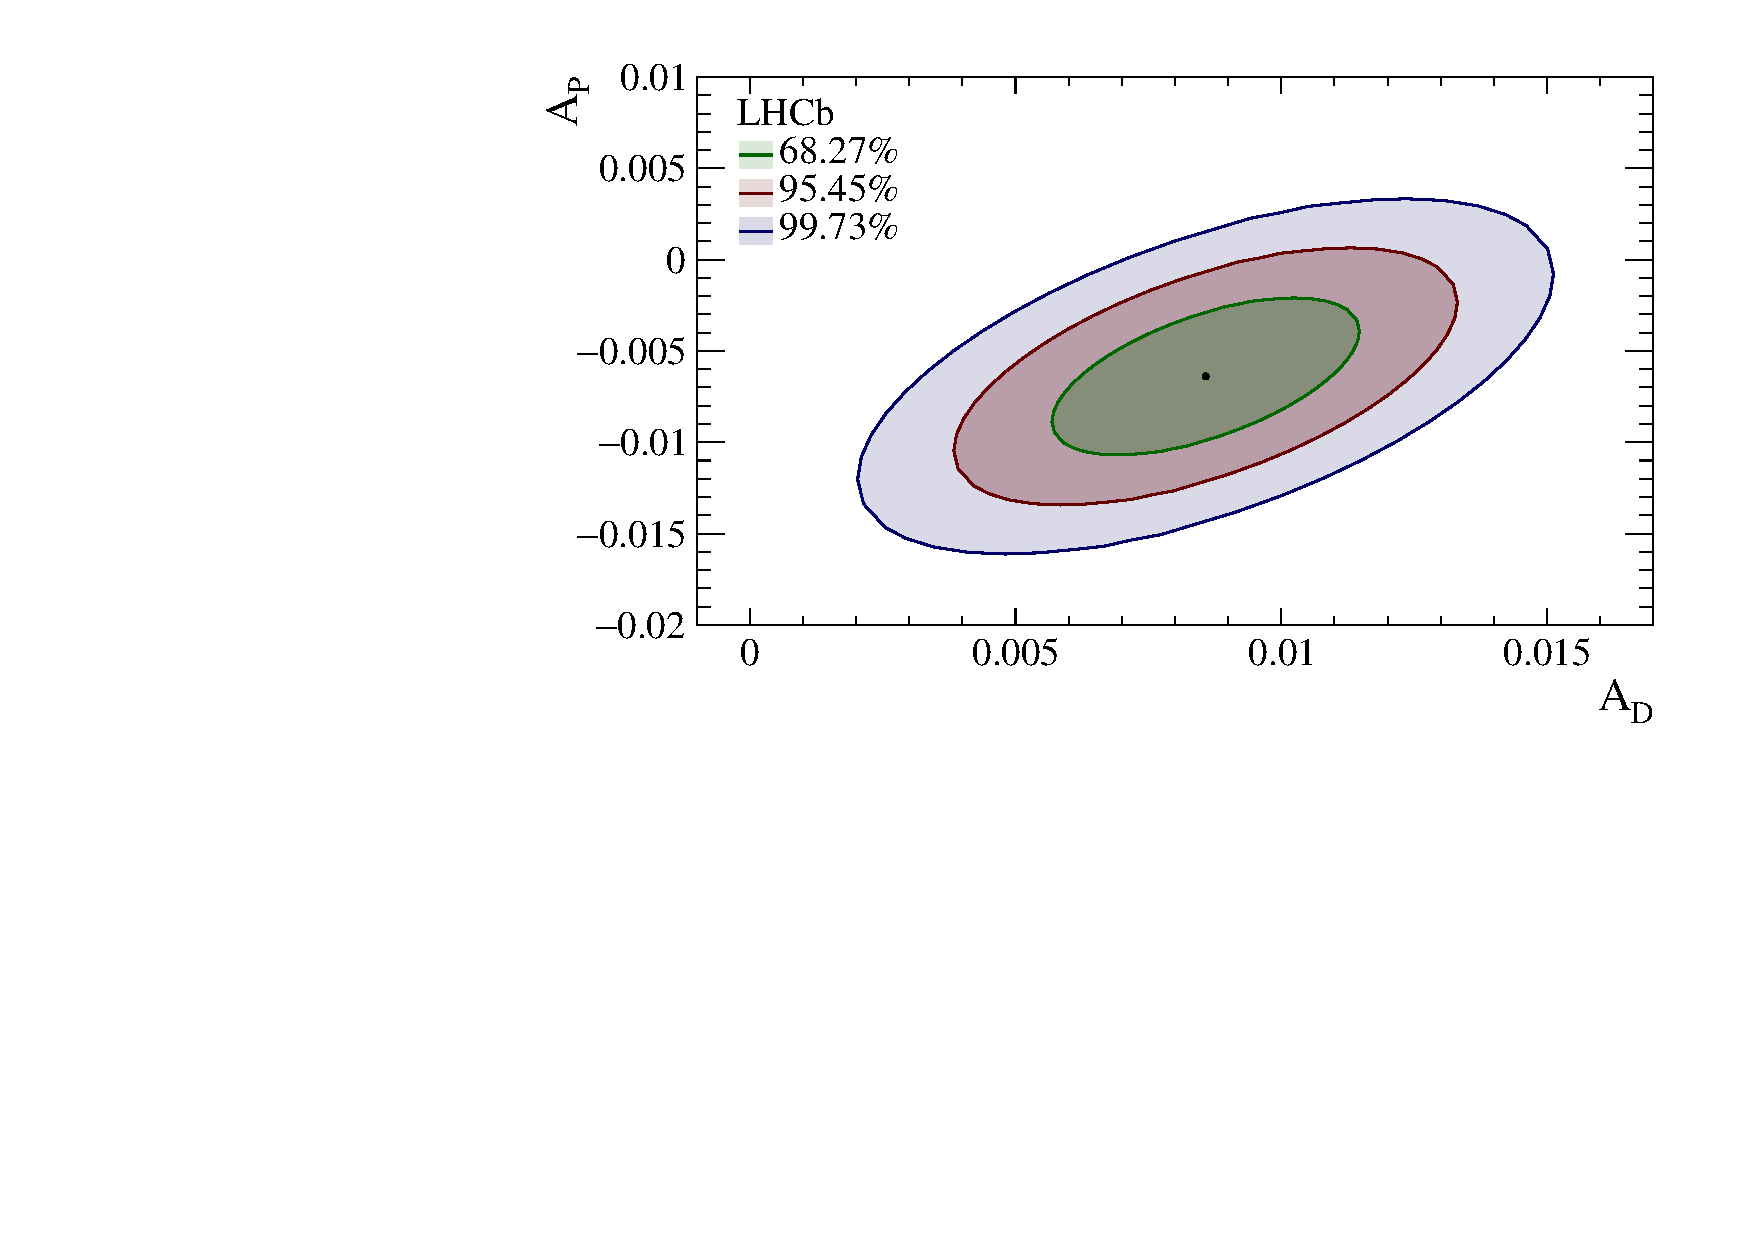
\includegraphics[width=0.48\linewidth]{05DecaytimeFit/figs/datafit/ADvsAP.pdf}
        \end{center}
        \vspace{-2mm}
        \caption{Plots for (\Sf, \Sfb) (left) and ($A_\mathrm{P}$, $A_\mathrm{D}$) (right) showing the one, two and three sigma contours.
        The shown uncertainties include the full statistical uncertainty and the systematic uncertainty due to the Gaussian constraints on
        the mixing frequency $\Delta m$ and the \Bz~decay width $\Gamma$.}
        \label{fig:timefitcCPcontour}
\end{figure}

Using the flavour tagging calibrations obtained from the fit, the tagging performance of the signal sample is computed.
The average of the total squared dilution is $(6.554\pm0.017)\%$. Taking
into account also untagged candidates, \ie~considering the tagging efficiency of $(85.23\pm0.05)\%$, the tagging power is $(5.59\pm0.01)\%$.
